\documentclass[]{kclthesis}

\modulecode{7CCSMPRJ} 
\submissiontitle{Individual Project Submission 2024-2025}
\studentnumber{K24087939}
\programme{Computational Finance M.Sc.}
\supervisor{Riaz Ahmad}
\wordcount{\red{Word count goes here}}
\title{Explainable Deep Learning for Portfolio Optimisation}
\author{Ingrid Pérez Aguilera}
\ReleaseProject{1} 
\department{Informatics} 

\usepackage{float}
\usepackage{hyperref}
\usepackage[utf8]{inputenc}
\usepackage{graphbox}
\usepackage{pgfgantt}
\usepackage{nomencl}
\usepackage[acronym]{glossaries}

\newtheorem{theorem}{Theorem}[section]
\newtheorem{exa}{Example}[section]
\newtheorem{corollary}[theorem]{Corollary}
\newtheorem{lemma}[theorem]{Lemma}
\newtheorem{proposition}[theorem]{Proposition}

\theoremstyle{definition}
\newtheorem{definition}[theorem]{Definition}
\newtheorem{remark}[theorem]{Remark}
\newtheorem{notation}[theorem]{Notation}
\newtheorem{assumption}[theorem]{Assumption}
\newtheorem{conjecture}[theorem]{Conjecture}

\newcommand{\ind}{1\hspace{-2.1mm}{1}} %Indicator Function
\newcommand{\I}{\mathtt{i}}
\newcommand{\D}{\mathrm{d}}
\newcommand{\E}{\mathrm{e}}
\newcommand{\RR}{\mathbb{R}}
\newcommand{\sgn}{\mathrm{sgn}}
\newcommand{\atanh}{\mathrm{arctanh}}
\def\blue#1{\textcolor{blue}{#1}}
\def\red#1{\textcolor{red}{#1}}

\setcounter{secnumdepth}{5}
\setlength{\marginparwidth}{2cm} % Adjust marginparwidth to avoid todonotes issues
\renewcommand{\contentsname}{Table of Contents}

\makeglossaries
\makenomenclature
\begin{document}
\pagenumbering{gobble}

%%%%% Cover page
\maketitle 

%%%%% Empty page
\newpage
\thispagestyle{empty}
\mbox{}
\newpage

%%%%% Abstract and acknowledgements
\chapter*{Abstract}

The dynamic and stochastic nature of financial markets together with the highly non-stationary and noisy financial time series data make the task of portfolio optimisation particularly challenging. However, it is their nature that makes them particularly well-suited for \acrfull{drl} algorithms, which can learn a trading strategy directly from the environment. Nonetheless, there are still significant challenges preventing its widespread adoption in the financial industry, such as difficulty in finding the appropriate algorithm with a suitable reward function and lack of transparency and interpretability. 

The goal of this thesis is to develop an explainable \acrshort{drl} model for portfolio optimisation that has the ability to leverage historical data to learn the optimal trading strategy that balances return maximisation and risk minimisation. Five prominent \acrshort{drl} algorithms are implemented and their performance is evaluated in different scenarios, including the impact of a larger financial environment representation, portfolio size and asset composition. Once the algorithms are trained, post-hoc explainability techniques are applied to understand which market conditions lead to a particular portfolio allocation.

Although the performance of the algorithms does not generally outperform all of the benchmarks, the results show that the agents are a powerful tool in portfolio management capable of learning from high-dimensional data and adapting to changing market conditions. The crucial contribution of this research lies in the explainability framework, particularly the use of \acrfull{shap} to provide insights into the decision-making process over the testing period in conjunction with interpretation for specific instances.  

\chapter*{Acknowledgements} 

I would like to express my gratitude to my supervisor, Dr. Riaz Ahmad, for his guidance and support throughout this project. I would also like to thank my Master's colleagues for being there during this journey and the valuable discussions we had.

I would like to convey my appreciation to my partner for his unwavering support and all the help in reviewing the code and the report. I would also like to acknowledge my family's continuous support and encouragement throughout my studies.

%%%%% Table of contents
\pagenumbering{roman}
\setcounter{tocdepth}{4}
\doublespacing
\tableofcontents
\newpage

%%%%% List of figures
\listoffigures
\newpage

%%%%% List of tables
\listoftables
\newpage

%%%%% Nomenclature
%% Numbers and Arrays
\nomenclature[A, 01]{$a$}{Scalar}
\nomenclature[A, 02]{$\mathbf{a}$}{Vector}
\nomenclature[A, 03]{$\mathbf{A}$}{Matrix}
\nomenclature[A, 04]{$\mathbf{1}$}{Matrix of $1$'s}

%% Sets
\nomenclature[B, 01]{$\mathbb{A}$}{Set}
\nomenclature[B, 02]{$\mathbb{R}$}{Set of real numbers}
\nomenclature[B, 03]{$[a, b]$}{Real interval including $a$ and $b$}
\nomenclature[B, 04]{$(a, b)$}{Real interval excluding $a$ and $b$}
\nomenclature[B, 05]{$[a, b)$}{Real interval including $a$ but excluding $b$}
\nomenclature[B, 06]{$(a, b]$}{Real interval excluding $a$ but including $b$}
\nomenclature[B, 07]{$\{0, 1\}$}{Set containing $0$ and $1$}
\nomenclature[B, 08]{$\{0, 1, ..., n\}$}{Set of all integers between $0$ and $n$ inclusive}
\nomenclature[B, 09]{$\emptyset$}{Empty set}
\nomenclature[B, 10]{$\mathbb{A}\subset\mathbb{B}$}{Set $\mathbb{A}$ is a proper subset of set $\mathbb{B}$}
\nomenclature[B, 11]{$\mathbb{A}\subseteq\mathbb{B}$}{Set $\mathbb{A}$ is a subset or equal to set $\mathbb{B}$}
\nomenclature[B, 12]{$\mathbb{A}\cap\mathbb{B}$}{Intersection of sets $\mathbb{A}$ and $\mathbb{B}$}
\nomenclature[B, 13]{$\mathbb{A}\cup\mathbb{B}$}{Union of sets $\mathbb{A}$ and $\mathbb{B}$}
\nomenclature[B, 14]{$\mathbb{A}\setminus\mathbb{B}$}{Set difference of sets $\mathbb{A}$ and $\mathbb{B}$}
\nomenclature[B, 15]{$|\mathbb{A}|$}{Cardinality of set $\mathbb{A}$}

%% Indexing
\nomenclature[C, 01]{$a_i$}{Element $i$ of vector $\mathbf{a}$, with indexing start at 1}
\nomenclature[C, 02]{$A_{i,j}$}{Element $i,j$ of matrix $\mathbf{A}$, with indexing start at 1}

%% Algebra Operations
\nomenclature[D, 01]{$\mathbf{A}^T$}{Transpose of matrix $\mathbf{A}$}
\nomenclature[D, 02]{$\mathbf{A}^{-1}$}{Inverse of matrix $\mathbf{A}$}

%% Probability
\nomenclature[E, 01]{$P(x)$}{Probability distribution over a random variable $x$}
\nomenclature[E, 02]{$P(x|y)$}{Conditional probability of $x$ given $y$}
\nomenclature[E, 03]{$E[x]$}{Expected value of random variable $x$}
\nomenclature[E, 04]{$Var[x]$}{Variance of random variable $x$}
\nomenclature[E, 05]{$Cov[x,y]$}{Covariance of random variables $x$ and $y$}
\nomenclature[E, 06]{$\mu$}{Mean}
\nomenclature[E, 07]{$\sigma$}{Standard deviation}
\nomenclature[E, 08]{$\sigma^2$}{Variance}
\nomenclature[E, 09]{$\Sigma$}{Covariance matrix}
\nomenclature[E, 10]{$\mathcal{N}(\mu, \sigma^2)$}{Normal distribution with mean $\mu$ and variance $\sigma^2$}
\nomenclature[E, 11]{$\mathcal{N}(0, 1)$}{Standard normal distribution}

%% Functions
\nomenclature[F, 01]{$f: \mathbb{A} \to \mathbb{B}$}{Function $f$ with domain $\mathbb{A}$ and range $\mathbb{B}$}
\nomenclature[F, 02]{$f(x)$}{Function $f$ evaluated at $x$}
\nomenclature[F, 03]{$f(x;\theta)$}{Function $f$ with parameters $\theta$ evaluated at $x$}
\nomenclature[F, 04]{$f'(x)$}{Derivative of function $f$}
\nomenclature[F, 05]{$\int f(x) \, dx$}{Integral of function $f$ with respect to $x$}
\nomenclature[F, 06]{$\min f(x)$}{Minimum of function $f$}
\nomenclature[F, 07]{$\min_x f(x)$}{Minimum of function $f$ with respect to $x$}
\nomenclature[F, 08]{$\max f(x)$}{Maximum of function $f$}
\nomenclature[F, 09]{$\max_x f(x)$}{Maximum of function $f$ with respect to $x$}
\nomenclature[F, 10]{$\log x$}{Natural logarithm of $x$}
\nomenclature[F, 11]{$x%!$}{Factorial of $x$}

%% Markov Decision Process
\nomenclature[G, 01]{$t$}{Time step}
\nomenclature[G, 02]{$\mathcal{S}$}{State space}
\nomenclature[G, 03]{$s_t$}{Observation of the state at time step $t$}
\nomenclature[G, 04]{$\mathcal{A}$}{Action space}
\nomenclature[G, 05]{$a_t$}{Action taken at time step $t$}
\nomenclature[G, 06]{$R(s,a,s')$}{Reward function}
\nomenclature[G, 07]{$r_t$}{Reward received at time step $t$}
\nomenclature[G, 08]{$T(s,a,s')$}{Transition function}
\nomenclature[G, 09]{$\gamma$}{Discount factor}
\nomenclature[G, 10]{$\pi$}{Policy}
\nomenclature[G, 11]{$G$}{Long-term reward}
\nomenclature[G, 12]{$V^\pi$}{State Value function for policy $\pi$}
\nomenclature[G, 13]{$Q^\pi$}{State-Action Value function for policy $\pi$}
\nomenclature[G, 14]{$A^\pi$}{Advantage function for policy $\pi$}

%% Other symbols
\nomenclature[Z]{$\forall$}{For all}
\nomenclature[Z]{$\in$}{Element of}
\nomenclature[Z]{$\nabla$}{Gradient}
\nomenclature[Z]{$\sum$}{Summation symbol}
\printnomenclature
\newpage

%%%%% List of acronyms
\newglossaryentry{financialmarkets}
{
    name=Financial Markets,
    text={financial markets},
    description={Marketplaces where people trade financial securities, commodities, and other fungible items of value at low transaction costs and at prices that reflect supply and demand}
}
\newglossaryentry{algorithmictrading}
{
    name=Algorithmic Trading,
    text={algorithmic trading},
    description={Use of computer algorithms to automate trading decisions and execute trades in financial markets}
}
\newglossaryentry{machinelearning}
{
    name=Machine Learning,
    description={Subset of artificial intelligence that enables systems to learn from data and improve their performance over time without being explicitly programmed}
}
\newglossaryentry{deeplearning}
{
    name=Deep Learning,
    description={Subset of machine learning that uses neural networks with many layers to learn from large amounts of data, enabling the model to automatically learn complex patterns and representations}
}
\newglossaryentry{reinforcementlearning}
{
    name=Reinforcement Learning,
    description={Subset of machine learning where an agent learns to make decisions by taking actions in an environment to maximise cumulative reward}
}
\newglossaryentry{deepreinforcementlearning}
{
    name=Deep Reinforcement Learning,
    description={Combination of deep learning and reinforcement learning, where deep neural networks are used to approximate the value function or policy in reinforcement learning tasks}
}
\newglossaryentry{artificialintelligence}
{
    name=Artificial Intelligence,
    description={Simulation of human intelligence processes by machines, especially computer systems, enabling them to perform tasks that typically require human intelligence, such as visual perception, speech recognition, decision-making, and language translation}
}
\newglossaryentry{explainableai}
{
    name=Explainable Artificial Intelligence,
    description={Methods and techniques in the application of artificial intelligence that make the results of the models understandable by humans, providing insights into how decisions are made}
}
\newglossaryentry{portfoliooptimisation}
{
    name=Portfolio Optimisation,
    text={portfolio optimisation},
    description={Process of selecting the best distribution of assets in a portfolio to achieve specific investment goals, such as maximising returns or minimising risk, while considering constraints and preferences}
}
\newglossaryentry{advantageactorcritic}
{
    name=Advantage Actor-Critic,
    description={Algorithm that uses both an actor (policy) and a critic (value function) to learn optimal policies by estimating the advantage of actions taken}
}
\newglossaryentry{proximalpolicyoptimization}
{
    name=Proximal Policy Optimization,
    description={Algorithm that optimises policies by ensuring that updates to the policy are not too large, maintaining a balance between exploration and exploitation}
}
\newglossaryentry{deepdeterministicpolicygradient}
{
    name=Deep Deterministic Policy Gradient,
    description={Algorithm that uses deep neural networks to learn policies for continuous action spaces, combining the benefits of deep learning and policy gradient methods}
}
\newglossaryentry{twindelayeddeepdeterministicpolicygradient}
{
    name=Twin Delayed Deep Deterministic Policy Gradient,
    description={Extension of \Gls{deepdeterministicpolicygradient} that addresses the overestimation bias in value function estimation by using two critic networks and delaying policy updates}
}
\newglossaryentry{softactorcritic}
{
    name=Soft Actor-Critic,
    description={Algorithm that combines the benefits of off-policy learning and entropy regularisation, allowing for more exploration and better stability in learning policies for continuous action spaces}
}
\newglossaryentry{shapleyadditiveexplanations}
{
    name=SHapley Additive exPlanations,
    description={Method for interpreting machine learning models by assigning each feature an importance value for a particular prediction, based on cooperative game theory}
}
\newglossaryentry{localinterpretablemodelagnosticexplanations}
{
    name=Local Interpretable Model-agnostic Explanations,
    description={Technique for explaining the predictions of any machine learning model by approximating it with a locally interpretable model, allowing users to understand the model's behaviour in a specific instance}
}
\newglossaryentry{featureimportance}{
    name=Feature Importance,
    description={Technique for determining the contribution of each feature in a machine learning model to its predictions, helping to identify which features are most influential}
}
\newglossaryentry{rewardfunction}{
    name=Reward Function,
    text={reward function},
    description={Function that defines the feedback signal received by an agent in reinforcement learning, guiding the agent's learning process by providing rewards or penalties based on its actions}
}
\newglossaryentry{hyperparameters}{
    name=Hyper-parameter,
    text={hyper-parameter},
    description={Parameter that is set before the learning process begins and control the learning process of a machine learning model, such as learning rate, batch size, and number of layers in a neural network}
}
\newglossaryentry{efficientfrontier}{
    name=Efficient Frontier,
    text={efficient frontier},
    description={Set of optimal portfolios that offer the highest expected return for a given level of risk, or the lowest risk for a given level of expected return, in the context of portfolio optimisation}
}
\newglossaryentry{modernportfoliotheory}{
    name=Modern Portfolio Theory,
    text={Modern Portfolio Theory},
    description={Investment theory that aims to construct a portfolio of assets that maximises expected return for a given level of risk, or minimises risk for a given level of expected return, through diversification}
}
\newglossaryentry{supervisedlearning}{
    name=Supervised Learning,
    description={Machine learning task where a model is trained on labelled data to learn a mapping from inputs to outputs}
}
\newglossaryentry{unsupervisedlearning}{
    name=Unsupervised Learning,
    description={Machine learning task where a model learns patterns or structures in unlabelled data without explicit supervision}
}
\newglossaryentry{deepneuralnetwork}{
    name=Deep Neural Network,
    text={deep neural network},
    description={Type of artificial neural network with multiple layers that can learn complex representations and patterns in data}
}
\newglossaryentry{markovdecisionprocess}{
    name=Markov Decision Process,
    text={Markov Decision Process},
    description={Mathematical framework for modelling decision-making in situations where outcomes are partly random and partly under the control of a decision maker, characterised by states, actions, rewards, and transition probabilities}
}
\newglossaryentry{partiallyobservablemarkovdecisionprocess}{
    name=Partially Observable Markov Decision Process,
    text={Partially Observable Markov Decision Process},
    description={Extension of \Gls{markovdecisionprocess} where the agent does not have access to the complete state information, requiring the use of belief states or observations to make decisions}
}
\newglossaryentry{bellmanequations}{
    name=Bellman Equations,
    text={Bellman equations},
    description={Set of equations that describe the relationship between the value of a state or action and the values of subsequent states or actions in dynamic programming and reinforcement learning, used to compute optimal policies} 
}

\newacronym{dl}{DL}{\Gls{deeplearning}}
\newacronym{ml}{ML}{\Gls{machinelearning}}
\newacronym{rl}{RL}{\Gls{reinforcementlearning}}
\newacronym{drl}{DRL}{\Gls{deepreinforcementlearning}}
\newacronym{a2c}{A2C}{\Gls{advantageactorcritic}}
\newacronym{ppo}{PPO}{\Gls{proximalpolicyoptimization}}
\newacronym{ddpg}{DDPG}{\Gls{deepdeterministicpolicygradient}}
\newacronym{td3}{TD3}{\Gls{twindelayeddeepdeterministicpolicygradient}}
\newacronym{sac}{SAC}{\Gls{softactorcritic}}
\newacronym{shap}{SHAP}{\Gls{shapleyadditiveexplanations}}
\newacronym{lime}{LIME}{\Gls{localinterpretablemodelagnosticexplanations}}
\newacronym{ai}{AI}{\Gls{artificialintelligence}}
\newacronym{xai}{XAI}{\Gls{explainableai}}
\newacronym{mpt}{MPT}{\Gls{modernportfoliotheory}}
\newacronym{dnn}{DNN}{\Glspl{deepneuralnetwork}}
\newacronym{mdp}{MDP}{\Gls{markovdecisionprocess}}
\newacronym{pomdp}{POMDP}{\Gls{partiallyobservablemarkovdecisionprocess}}

\printglossary
\printglossary[type=\acronymtype]
\newpage

%%%%% Main content
\pagenumbering{arabic}
\onehalfspacing
\setlength{\parindent}{0pt}
\setlength{\parskip}{6pt}


%%%%%% Chapters
\doublespacing
\section{Glossaries and Acronyms Sample use}
The \Gls{latex} typesetting markup language is specially suitable for documents that include \gls{maths}. 

Given a set of numbers, there are elementary methods to compute its \acrlong{gcd}, which is abbreviated \acrshort{gcd}. This  process is similar to that used for the \acrfull{lcm} \cite{Doe11}.

\chapter{Introduction} \label{ch:introduction}

\Gls{financialmarkets} are highly complex systems influenced by numerous factors, including economic and political events, social trends and technological advancements. Moreover, their evolving and stochastic nature requires using the most advance computational developments to model the financial environment. The tasks of financial time series prediction and \gls{portfoliooptimisation} are considerably intricate, due to the semi-strong form of market efficiency and the high level of noise. \cite{Shen2020}

\Gls{algorithmictrading} focuses on the application of analytical methods to automatically execute trading actions based on an algorithm without human intervention. Initially, the field mainly studied the usage of a computer program to follow a predefined strategy \cite{Lei2020}. More recently, algorithmic trading involves environment perception by learning feature representation from highly non-stationary and noisy financial time series data, and decision-making by exploring the environment and simultaneously taking actions without supervision \cite{Ma2021}.

\acrfull{ml} has an advantage for the task due to its ability to learn from historical data and make predictions about the future state of an environment. Research has explored the application of \acrfull{dl} in future price prediction of financial assets \cite{Hasan2024,Nti2020,Shen2020,Wu2023}. However, its main disadvantage is the inability to directly handle trading, requiring an additional step to convert the predictions into actionable strategies. In contrast, \acrfull{rl} allows the algorithm to learn a trading strategy directly from the environment, without the need for a separate step \cite{Moody2001,Yang2020}. In this case, there are two main approaches: first, the algorithm can learn the amount of assets to buy, sell or hold at each time step \cite{Liu2018}, or second, the algorithm can learn the optimal portfolio allocation and automatically rebalance the portfolio weights at each time step \cite{Guan2021}.

Despite the potential of \acrshort{rl} in portfolio optimisation, its widespread adoption in the financial industry remains limited. This is primarily due to following challenges \cite{Cortes2024}:
\begin{enumerate}
    \item difficulty in finding the appropriate algorithm with a suitable \gls{rewardfunction} and \glspl{hyperparameters} to ensure efficiency and performance,
    \item challenge of testing the algorithm in a real-world environment, and
    \item lack of transparency of \acrshort{ml} models, often referred to as \glspl{blackbox}, making it increasingly intractable to interpret the algorithm's decisions.
\end{enumerate}

In recent years, the rise in popularity of \acrfull{ai} and its widespread use have led to concerns regarding its decisions due to its \gls{blackbox} nature \cite{Bathaee2018TheAI}. The concept of explainability in \acrshort{ai}, known as \acrfull{xai}, refers to a model's ability to provide details and reasons to make itself understandable \cite{BarredoArrieta2019}. The term was first coined in 2016 to describe the need for users to effectively understand, trust and manage artificial intelligence applications \cite{Gunning2019}. The need for explainability becomes particularly relevant within the financial domain, where the regulatory framework requires transparency and accountability in automated decision-making. Various relevant applications, including volatility models \cite{Brigo2021}, credit risk assessment \cite{GarciaCespedes2025} and portfolio construction \cite{Cortes2024}, have explored the concept of explainability in financial applications. 

Consequently, this thesis will focus on addressing the aforementioned challenges by exploring the application of \acrfull{drl} to portfolio optimisation and implementing explainability techniques to understand model behaviour.

\section{Objectives} \label{sec:introduction-objectives}

The objective of this thesis is to develop an explainable \acrshort{drl} model for portfolio optimisation. A \acrshort{drl} model has the ability to leverage historical financial data to learn an investment strategy that efficiently allocates financial assets while maximising expected returns and minimising risk. Moreover, the incorporation of advanced explainability techniques enhances the interpretability and transparency of the model's decision-making. This project aims to bridge the gap between cutting-edge machine learning techniques and their practical application in finance by addressing the challenges of algorithm selection, simulation of real-world scenarios, and \gls{blackbox} nature of \acrshort{ml} models.

First, \acrshort{drl} models, namely \acrfull{a2c}, \acrfull{ppo}, \acrfull{ddpg}, \acrfull{td3} and \acrfull{sac}, will be employed to learn the optimal portfolio allocation from high-dimensional environment representations. The algorithms will be trained on historical financial data, including technical and macroeconomic indicators, with the goal of capturing the complex market dynamics. Each of the algorithms is better suited to a particular scenario, for instance, \acrshort{ddpg} encourages maximum returns \cite{Lillicrap2015}, while \acrshort{a2c} reduces the variance \cite{Mnih2016} and \acrshort{ppo} is better at balancing \gls{exploration} versus \gls{exploitation} \cite{Schulman2017}.

Second, post-hoc explainability techniques: \Gls{featureimportance}, \acrfull{lime} and \acrfull{shap} will be applied to interpret the model's decisions. The goal of these is to understand which market conditions, represented by financial data, lead to the actions/decisions, encoded as portfolio weights. 

Finally, the performance of the \acrshort{drl} models will be analysed in different scenarios, including the impact of a larger financial environment representation, portfolio size and asset composition. The results will be compared with traditional portfolio optimisation methods to evaluate the effectiveness of the proposed approach.

\section{Report Structure} \label{sec:introduction-structure}

This report is organised into six chapters, each of which focuses on a concrete area related to the problem. Additional material, together with source code, is included in the appendices. 

The current chapter, \ref{ch:introduction}, presents the motivation and the objectives of this thesis. It gives an overview of the potential of \acrshort{drl} in portfolio optimisation and its main challenges, particularly the lack of transparency of \acrshort{ml} models. 

Chapter \ref{ch:background} provides an overview of the theoretical background of the project. The problem of financial portfolio optimisation is outlined and the potential of \acrshort{drl} in this context is discussed. The chapter provides a comprehensive background explanation of the fundamentals of \acrlong{dl} and \acrlong{rl}, including the main algorithms (\acrshort{a2c}, \acrshort{ppo}, \acrshort{ddpg}, \acrshort{td3}, \acrshort{sac}). In addition, it gives an overview of the post-hoc explainability techniques (\Gls{featureimportance}, \acrshort{lime} and \acrshort{shap}) used to interpret the model's decisions. Finally, it includes a comprehensive in-depth literature review on the topics of \acrshort{ml} applied to portfolio optimisation and relevant applications of explainability techniques. 

The methodology, chapter \ref{ch:methodology}, describes the techniques and methods used and outlines the implementation of the proposed solution. The chapter provides a detailed explanation of the architecture and components of the proposed \acrshort{drl} model, including the state representation and reward function. Furthermore, given the trained algorithms, it describes the implementation of the post-hoc explainability techniques.

The results of the experiments are presented in chapter \ref{ch:results}, which analyses and evaluates the performance of the proposed methodology, while critically discussing the findings. It provides a detailed comparison of the \acrshort{drl} strategies with traditional portfolio optimisation methods. Furthermore, it consists of an analysis of the model's decisions using post-hoc explainability techniques.

Chapter \ref{ch:issues} discusses the legal, social, ethical and professional implications within the context of the project. By addressing these issues, the project aims to ensure that the proposed solution adheres to industry standards, while considering the implications of the technology.

Finally, the report concludes with a summary of the main points of the work, the contributions made, in conjunction with potential applications and future work in chapter \ref{ch:conclusion}.

\chapter{Background} \label{ch:background}

This chapter provides an overview of the problem of portfolio optimisation in the financial domain, followed by a comprehensive explanation of the fundamentals of \acrfull{dl} and \acrfull{rl}, including the relevant algorithms in the field of \acrfull{drl}. In addition, it discusses the need for explainability in \acrfull{ml} and the main techniques used to achieve it: \acrfull{shap}, \acrfull{lime} and \Gls{featureimportance}. Finally, it presents the state of the art in portfolio optimisation using \acrshort{drl} and the recent advancements in explainability techniques in the field. 

\section{Portfolio Optimisation} \label{sec:portfoliooptimisation}

\Gls{portfoliooptimisation} is the process of selecting optimal weights for a portfolio of assets in order to maximise expected returns for a given level of risk, or conversely, to minimise risk for a given level of expected returns \cite{Sato2019}. In mathematical terms, the problem requires finding a solution to the specified objective function, which is typically a function of the expected returns and the risk associated with the portfolio \cite{Bruce2014}. The task becomes further complicated if a time dimension is introduced, as the portfolio weights need to be adjusted over time to capture the changes in market conditions and asset prices \cite{Li2019}. 

\subsection{Modern Portfolio Theory}

There exist several traditional frameworks that formalise the problem of portfolio allocation. Markowitz's \acrfull{mpt} was proposed in 1952 \cite{Markowitz1952} and it provides a mathematical framework where investors choose optimal portfolios based on risk and return, by either minimising the risk given a specified return or, maximising the return given a specified risk \cite{kent}. The theory extends the concept of diversification by suggesting that owning financial assets of different kinds is less risky than owning assets of the same kind, due to the correlations between assets. 

The main assumptions in \acrshort{mpt} are:
\begin{itemize}
    \item investors are risk-averse, rational, and seek to maximise return for a given risk;
	\item returns are normally distributed;
	\item markets are frictionless, meaning there are no transaction costs; and
	\item assets are infinitely divisible.
\end{itemize}

Under these assumptions, portfolio risk and return can be modelled as an optimisation problem. Let $\mathbf{w} = \left(w_1, w_2, \dots, w_N\right)^T$ denote the portfolio weight vector, where each $w_i$ indicates the proportion of capital allocated to asset $i$, subject to the budget constraint:
\begin{equation}
    \sum_{i=1}^{N} w_i = 1 \quad \Leftrightarrow \quad \mathbf{w}^T \mathbf{1} = 1
\end{equation}
with $\mathbf{1} \in \mathbb{R}^N$ being a vector of ones, and subject to the non-negativity constraint, meaning that short-selling is not allowed:
\begin{equation}
    w_i \geq 0 \quad \forall i = 1, 2, \dots, N.
\end{equation}

Let $\boldsymbol{\mu} = \left(R_1, R_2, \dots, R_N\right)^T$ represent the vector of expected returns, and $\Sigma \in \mathbb{R}^{N \times N}$ the covariance matrix of asset returns. The expected return of the portfolio is then given by:
\begin{equation}
    R_p = \mathbf{w}^T \boldsymbol{\mu},
\end{equation}
and the portfolio risk is quantified by the variance of returns:
\begin{equation}
    \sigma_p^2 = \mathbf{w}^T \Sigma \mathbf{w}.
\end{equation}

This formulation provides the foundation for solving the mean-variance optimisation problem, by either:
\begin{itemize}
    \item minimising portfolio variance $\sigma_p^2$ subject to a target expected return $R_p$, or
    \item maximising expected return $R_p$ subject to a risk constraint $\sigma_p$.
\end{itemize}

The Markowitz mean-variance optimisation problem can be expressed as:
\begin{equation}
\begin{aligned}
    \min_{\mathbf{w}} \quad & \mathbf{w}^T \Sigma \mathbf{w} \\
    \text{subject to} \quad &
    \begin{cases}
        \mathbf{w}^T \boldsymbol{\mu} = R_p \\
        \mathbf{w}^T \mathbf{1} = 1 \\
        \mathbf{w} \geq 0
    \end{cases}
\end{aligned}
\end{equation}

Solving the mean-variance optimisation problem for varying levels of target return leads to a set of optimal portfolios that form the \gls{efficientfrontier}. It is typically visualised in a risk-return space, where the x-axis represents the risk (standard deviation) and the y-axis represents the expected return, as shown in Figure \ref{fig:efficient_frontier}. Portfolios below the curve are suboptimal, while those on the frontier represent the best achievable combinations of risk and return.

\begin{figure}[ht]
    \centering
    \includegraphics[width=0.8\textwidth]{figures/markowitz-efficient-frontier.png}
    \caption{Efficient Frontier in Risk-Return Space. \cite{Bodie2014}}
    \label{fig:efficient_frontier}
\end{figure}

Despite the simplicity in the formulation of \acrshort{mpt}, its assumptions do not reflect the behaviour of real markets. Moreover, modern markets are dynamic, non-stationary, and feature non-linear relationships, which have driven research into other approaches better suited to capture the complexities of modern financial markets. 

\section{Deep Reinforcement Learning} \label{sec:deepreinforcementlearning}

\acrfull{drl} is a sub-field of \acrfull{dl} that combines \acrfull{dl} and \acrfull{rl} to solve sequential decision-making problems with high-dimensionality in the environment representation. This approach has gained significant attention in recent years due to its success in various applications, including robotics \cite{Tang2024} and game playing \cite{Silver2016, Shao2019}.

\acrlong{ml} is a branch of \acrfull{ai} that focuses on the use of data and algorithms to imitate the way humans learn, gradually improving their accuracy over time \cite{IBM2021}. There are three main tasks in \acrshort{ml} \cite{Francois-Lavet2018}:

\begin{itemize}
    \item \textbf{\Gls{supervisedlearning}}: Task of inferring a classification or regression from labelled training data, where the model learns to map inputs to outputs based on examples.
    \item \textbf{\Gls{unsupervisedlearning}}: Task of drawing inferences from datasets consisting of unlabelled input data, where the model learns to identify patterns or structures in the data.
    \item \textbf{\acrlong{rl}}: Task of training an agent to sequentially make decisions by taking actions in an environment with the goal of maximising cumulative reward, using feedback from the environment to learn.
\end{itemize}

Consequently, \acrshort{rl} emerges as a framework for solving complex decision-making problems, where an agent continuously interacts with an environment, receiving observations about its states and rewards based on the actions taken. The agent's objective is to learn a policy that maximises the expected cumulative reward over time.

Conversely, \acrlong{dl} is not a \acrshort{ml} task, but rather a set of methods and techniques to solve such \acrshort{ml} tasks, specially in supervised and unsupervised learning tasks. \acrshort{dl} focuses on the use of \acrfull{dnn} \cite{Goodfellow2016}, which are characterised by a succession of layers of non-linear transformation that allow the model to learn a representation of the data with various levels of abstraction.

\subsection{Reinforcement Learning} \label{sec:reinforcementlearning}

As mentioned, \acrshort{rl} is a type of \acrshort{ml} that solves the problem of sequential decision-making through continuous interaction with an environment. The agent learns to take actions given a representation of the environment's state with the goal of optimising a pre-defined notion of reward. The agent learns by successively adjusting its policy based on its observations and interactions with the environment. 

The \acrshort{rl} problem can be formalised as a discrete-time stochastic control process where an agent interacts with the environment. At each time step $t$, the agent observes the state of the environment $s_t \in \mathcal{S}$, takes an action $a_t \in \mathcal{A}$ to obtain a reward $r_t \in \mathbb{R}$ and transition to a new state $s_{t+1} \in \mathcal{S}$, where $\mathcal{S}$ is the state space and $\mathcal{A}$ is the action space \cite{Francois-Lavet2018}. The agent's interaction with the environment is visually represented in Figure \ref{fig:agent_environment_interaction}.

\begin{figure}[ht]
    \label{fig:agent_environment_interaction}
    \centering
    \begin{tikzpicture}[>=stealth]
    % Nodes
    \node[draw, rectangle, minimum width=2cm, minimum height=1cm] (agent) {Agent};
    \node[draw, rectangle, minimum width=2.8cm, minimum height=1cm, right=5cm of agent] (env) {Environment};

    % Coordinates for paths
    \coordinate (top1) at ($(env.north)+(0,1.5)$);
    \coordinate (top2) at ($(agent.north)+(0,1.5)$);

    \coordinate (bot1) at ($(env.south)+(0,-1.5)$);
    \coordinate (bot2) at ($(agent.south)+(0,-1.5)$);

    % Arrows
    \draw[->] (agent) -- node[above, midway] {Action $a_t$} (env);
    \draw[->] (env.north) -- (top1) -- node[above] {State $s_t$} (top2) -- (agent.north);
    \draw[->] (env.south) -- (bot1) -- node[below] {Reward $r_t$} (bot2) -- (agent.south);
\end{tikzpicture}
    \caption{Agent interaction with environment}
\end{figure}

A discrete time stochastic control process can be formalised as a \acrfull{mdp}, if it fulfils the Markov Property. 

\begin{definition}[Markov Property]
    A discrete time stochastic control process satisfies the Markov Property if:
    \begin{eqnarray}
        P(s_{t+1} | s_t, a_t) = P(s_{t+1} | s_t, a_t, s_{t-1}, a_{t-1}, \dots, s_0, a_0) \\  
        P(r_t | s_t, a_t) = P(r_t | s_t, a_t, s_{t-1}, a_{t-1}, \dots, s_0, a_0)
    \end{eqnarray}
    where $P(s_{t+1} | s_t, a_t)$ is the transition probability of moving to state $s_{t+1}$ given the current state $s_t$ and action $a_t$, and $P(r_t | s_t, a_t)$ is the reward function that defines the expected reward received at time $t$ given the current state and action.
\end{definition}

This implies that the state $s_{t+1}$ at a future time step $t+1$ only depends on the current state $s_t$ and action $a_t$. Similarly, the reward $r_t$ at time step $t$ only depends on the current state and action and not on the history of previous states and actions. Consequently, a \acrlong{mdp} \cite{Bellman1957} is a discrete time stochastic control process defined as:

\begin{definition}[Markov Decision Process]
    An \acrshort{mdp} is a tuple $\mathcal{M} = \left(\mathcal{S}, \mathcal{A}, T, R, \gamma\right)$, where:
    \begin{itemize}
        \item $\mathcal{S}$ is the state space: $s_t \in \mathcal{S}$,
        \item $\mathcal{A}$ is the action space: $a_t \in \mathcal{A}$,
        \item $T: \mathcal{S} \times \mathcal{A} \times \mathcal{S} \rightarrow [0, 1]$ is the transition function,
        \item $R: \mathcal{S} \times \mathcal{A} \times \mathcal{S} \rightarrow \mathcal{R}$ is the reward function, where $\mathcal{R} \in \left[0, R_{max}\right]$ is the set of all possible rewards bounded by $R_{max} \in \mathbb{R}^+$, and
        \item $\gamma \in [0, 1)$ is the discount factor.
    \end{itemize}
    
\end{definition}

At each time step, the probability of advancing to the next state $s_{t+1}$ is given by the transition function $T(s_t, a_t, s_{t+1})$ and the reward $r_t$ is given by the reward function $R(s_t, a_t, s_{t+1})$. This can be visualised in Figure \ref{fig:mdp}.

\begin{figure}[ht]
    \label{fig:mdp}
    \centering
    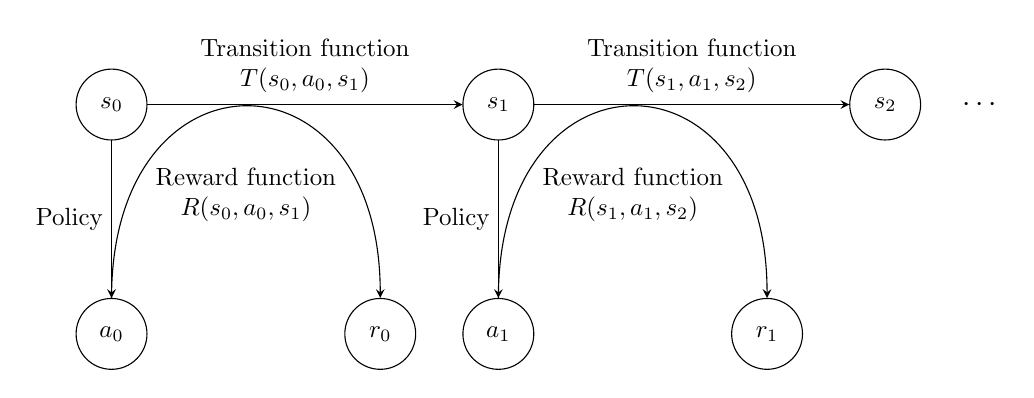
\begin{tikzpicture}[->, >=stealth, node distance=2cm, every node/.style={scale=0.9}]
    % State nodes
    \node[circle, draw, minimum size=1cm] (s0) {$s_0$};
    \node[circle, draw, minimum size=1cm, right=4cm of s0] (s1) {$s_1$};
    \node[circle, draw, minimum size=1cm, right=4cm of s1] (s2) {$s_2$};

    % Action nodes
    \node[circle, draw, minimum size=1cm, below=2cm of s0] (a0) {$a_0$};
    \node[circle, draw, minimum size=1cm, below=2cm of s1] (a1) {$a_1$};

    % Reward nodes
    \node[circle, draw, minimum size=1cm, right=2.5cm of a0] (r0) {$r_0$};
    \node[circle, draw, minimum size=1cm, right=2.5cm of a1] (r1) {$r_1$};

    % Arrows between states
    \draw[->] (s0) -- (s1) node[midway, above] {\begin{tabular}{c}
            Transition function \\
            $T(s_0, a_0, s_1)$
        \end{tabular}};
    \draw[->] (s1) -- (s2) node[midway, above] {\begin{tabular}{c}
            Transition function \\
            $T(s_1, a_1, s_2)$
        \end{tabular}};

    % Policy arrows 
    \draw[->] (s0) -- (a0) node[midway, left] {Policy};
    \draw[->] (s1) -- (a1) node[midway, left] {Policy};

    \draw[->] (a0) .. controls +(0,3.7) and +(0,3.7) .. node[midway, below, yshift=-20pt] {\begin{tabular}{c}
            Reward function \\
            $R(s_0, a_0, s_1)$
        \end{tabular}} (r0);

    \draw[->] (a1) .. controls +(0,3.7) and +(0,3.7) .. node[midway, below, yshift=-20pt] {\begin{tabular}{c}
            Reward function \\
            $R(s_1, a_1, s_2)$
        \end{tabular}} (r1);

    % Ellipsis
    \node at ($(s2)+(1.2cm,0)$) {\large $\cdots$};

\end{tikzpicture}
    \caption{Markov Decision Process with policy, transition, and reward functions}
\end{figure}

The agent's objective is to learn a policy $\pi: \mathcal{S} \rightarrow \mathcal{A}$ that maps states to actions, in order to maximise the expected cumulative reward over time. Policies can be categorised as:
\begin{itemize}
    \item deterministic: $\pi(s) : \mathcal{S} \to \mathcal{A}$, at a given state $s$, the policy specifies the only available action to take, or
    \item stochastic: $\pi(s, a) : \mathcal{S} \times \mathcal{A} \to [0, 1]$, at a given state $s$, the policy specifies the probability of taking action $a$.
\end{itemize}

\acrlong{mdp} are based on the idea that the current state is fully representative of the environment. However, in most real world scenarios, the agent does not have access to the complete state. In such cases, \acrfull{pomdp} can be used to model the uncertainty in the agent's observations and actions.

The goal of the agent is to maximise the cumulative long-term reward $G_t$, which is defined as the sum of discounted rewards over time:
\begin{equation}
    G_t = r_{t+1} + \gamma r_{t+2} + \gamma^2 r_{t+3} + \dots = r_{t+1} + \gamma G_{t+1}
\end{equation}
where $\gamma \in [0, 1)$ is the discount factor and is used to balance the importance between immediate and future rewards. If the discount factor is set to 0, the agent is myopic and only maximises the immediate reward; whereas, as $\gamma$ approaches $1$, the agent becomes more far-sighted and places greater importance on future rewards.

The expected cumulative reward is defined as the state value function $V^\pi(s): \mathcal{S} \to \mathbb{R}$, which is the expected return when starting from state $s$ and following policy $\pi$:
\begin{equation}
    V^\pi(s) = \mathbb{E}_\pi \left[G_t | s_t = s\right] 
\end{equation}
where $\mathbb{E}_\pi$ denotes the expectation over the policy $\pi$.

Similarly, the state-action value function $Q^\pi(s, a): \mathcal{S} \times \mathcal{A} \to \mathbb{R}$ is defined as the expected return when starting from state $s$, taking action $a$, and then following policy $\pi$:
\begin{equation}
    Q^\pi(s, a) = \mathbb{E}_\pi \left[G_t | s_t = s, a_t = a\right] 
\end{equation}

The state value function $V^\pi(s)$ and the state-action value function $Q^\pi(s, a)$ are related as follows:
\begin{equation}
    V^\pi(s) = \sum_{a \in \mathcal{A}} \pi(a | s) Q^\pi(s, a) = \mathbb{E}_\pi \left[Q^\pi(s, a) \mid s_t = s\right]
\end{equation}

A policy $\pi$ is said to be optimal if the policy's value function is the optimal value function of the \acrshort{mdp}, defined as: 
\begin{eqnarray}
    V^*(s) = \max_{\pi'} V^{\pi'}(s), \forall s \in \mathcal{S} \\ 
    Q^*(s, a) = \max_{\pi'} Q^{\pi'}(s, a), \forall s \in \mathcal{S}, a \in \mathcal{A}
\end{eqnarray}
The optimal policy $\pi^*$ is:
\begin{equation}
    \pi^*(s) = \arg \max_{a\in \mathcal{A}} Q^*(s, a)
\end{equation}

As a result, the optimal policy is the greedy policy that performs the optimal actions at each time step as determined by the optimal value functions. This enables the agent to determine optimal actions that maximise long-term returns by evaluating immediate information, without requiring knowledge of the values of future states and actions.

The \Gls{bellmanequations} \cite{Bellman1957book} provide a recursive relation between the value functions in terms of the future state/action values. There are four main Bellman equations, classified in two groups: the Bellman expectation equations and the Bellman optimality equations. The Bellman expectation equations are defined as follows:
\begin{eqnarray}
    V^\pi(s) = \sum_{a \in \mathcal{A}} \pi\left(a \mid s\right) \sum_{s'\in \mathcal{S}} T\left(s, a, s'\right) \left[R\left(s,a\right) + \gamma V^\pi(s')\right] \\ 
    Q^\pi(s, a) = \sum_{s'\in \mathcal{S}} T\left(s, a, s'\right) \left[R\left(s,a\right) + \gamma \sum_{a' \in \mathcal{A}} \pi\left(a' \mid s'\right) Q^\pi(s', a')\right]
\end{eqnarray}

and the Bellman optimality equations are defined as:
\begin{eqnarray}
    V^*(s) = \max_{a \in \mathcal{A}} \sum_{s'\in \mathcal{S}} T\left(s, a, s'\right) \left[R\left(s,a\right) + \gamma V^*(s')\right] \\
    Q^*(s, a) = \sum_{s'\in \mathcal{S}} T\left(s, a, s'\right) \left[R\left(s,a\right) + \gamma \max_{a' \in \mathcal{A}} Q^*(s', a')\right]
\end{eqnarray}

Although explicitly solving the Bellman equations would lead to the optimal policy, it is often intractable due to the size of the state and action spaces. Therefore, in \acrshort{rl} algorithms, the goal is to learn an approximation of the optimal value functions, which can be used to derive the optimal policy. Another problem that arises is that of balancing exploration and exploitation \cite{Thrun1992}. Theoretically, following the greedy action yields the optimal policy, but this is only true if the action values are known. In practice, the agent at each time step and given state chooses either an action whose value is higher, thus exploiting the current knowledge, or picks an action at random, thus exploring the environment and gaining more information about the state-action space, leading to potentially discovering a better action than the greedy one.


\chapter{Methodology} \label{ch:methodology}

This chapter covers the methodology and framework established to provide an explainable \acrfull{drl} model capable of optimising a portfolio of financial assets. The chapter is structured as follows: first, it describes the architecture and components of the proposed \acrshort{drl} model, including the state representation, reward function and training process. Second, it discusses the evaluation metrics and experimental setup used to assess the performance of the proposed solution. Finally, it outlines the implementation of the explainability techniques used to interpret the model's decisions. 

\section{Problem Definition} \label{sec:problem-definition}

The problem of \gls{portfoliooptimisation} is the task of finding an optimal allocation of financial assets in a portfolio to maximise expected returns while minimising risk. Thus, it is necessary to decide how to rebalance the portfolio at each time step in a highly stochastic and complex financial market. This can be formulated using a \acrfull{mdp} framework, where the agent interacts with the environment by deciding the optimal allocation based on the state of the environment at each time step to maximise the expected cumulative reward over time. \acrfull{drl} gives the agent the ability to learn the optimal policy directly from the environment by taking actions and receiving rewards. 

\section{Markov Decision Process Model} \label{sec:mdp-model}

Due to the dynamic, stochastic and interactive nature of financial markets, a \acrlong{mdp} is a suitable framework to model the problem. The main elements of the \acrshort{mdp} model are defined as follows:
\begin{itemize}
    \item State space $\mathcal{S}$
    \item Action space $\mathcal{A}$
    \item Reward function $R: \mathcal{S} \times \mathcal{A} \times \mathcal{S} \to \mathbb{R}$
    \item Transition function $T: \mathcal{S} \times \mathcal{A} \to \mathcal{S}$
    \item Discount factor $\gamma \in [0,1)$
\end{itemize}

The state space $\mathcal{S}$ is a vector representation of the financial environment. For a portfolio of $D$ assets, the features that describe the state include asset prices, technical indicators and macroeconomic indicators: 
\begin{itemize}
    \item Close price $\mathbf{p}_t \in \mathbb{R}^D$: Adjusted close prices of the assets at time $t$.
    \item Open price $\mathbf{o}_t \in \mathbb{R}^D$: Opening prices of the assets at time $t$.
    \item High price $\mathbf{h}_t \in \mathbb{R}^D$: Highest prices of the assets at time $t$.
    \item Low price $\mathbf{l}_t \in \mathbb{R}^D$: Lowest prices of the assets at time $t$.
    \item Volume $\mathbf{v}_t \in \mathbb{R}^D$: Trading volume of the assets at time $t$.
    \item Technical indicators $\mathbf{I}_t \in \mathbb{R}^{D \times I}$: For each of the $D$ assets, a vector $\mathbf{i}_t$ of $I$ technical indicators, such as moving averages, relative strength index (RSI), and Bollinger Bands, calculated from the asset prices.
    \item Macroeconomic indicators $\mathbf{M}_t \in \mathbb{R}^{D \times M}$: For each of the $D$ assets, a vector $\mathbf{m}_t$ of $M$ macroeconomic indicators, such as volatility index and interest rates, which provide additional context about the financial environment.
    \item Covariance matrix $\mathbf{C}_t \in \mathbb{R}^{D \times D}$: For each of the $D$ assets, a vector of $D$ values representing the covariance between the assets in the portfolio at time $t$.
\end{itemize}

The description of technical and macroeconomic indicators is provided in more detail in Appendix \ref{app:state_representation}.

The action space $\mathcal{A}$ is the set of possible actions that the agent can take at each time step. For the portfolio optimisation problem, the actions correspond to portfolio weights and are defined as follows:
\begin{equation}
    \mathbf{a}_t = \mathbf{w}_t : w_{t,d} \in [0, 1] \quad \forall d \in \{1, \ldots, D\},
\end{equation}
where $\mathbf{w}_t$ is a vector of portfolio weights at time $t$, representing the allocation of the portfolio to each asset. The weights are constrained to be non-negative and sum to one:
\begin{equation}
    \sum_{d=1}^D w_{t,d} = 1, \quad w_{t,d} \geq 0 \quad \forall d \in \{1, \ldots, D\}.
\end{equation}
Moreover, they are initialised to be equal for all assets, meaning that the agent starts with an equal allocation to each asset in the portfolio. The reason behind this is to avoid an initial bias and allow the agent to learn an allocation from the environment rather than favour any particular asset.

The transition function $T$ describes how the state of the environment changes in response to the action taken. It is defined as:
\begin{equation}
    s_{t+1} = T(s_t, a_t),
\end{equation}
where $s_{t+1}$ is the new state of the environment after taking action $a_t$ in state $s_t$. The transition function is determined by the dynamics of the financial market, which are influenced by the asset prices, trading volume and other factors.

The reward function $R$ models the direct reward of taking an action $a_t$ in state $s_t$ and transitioning to a new state $s_{t+1}$. It is defined as the change in the portfolio value from time $t$ to time $t+1$:
\begin{equation}
    R_{t+1} = R(s_t, a_t, s_{t+1}) = V_{t+1} - V_t,
\end{equation}
where the value of the portfolio at time $t$ is given by the dot product of the portfolio weights and the asset close prices:
\begin{equation}
    V_t = \mathbf{w}_t \cdot \mathbf{p}_t.
\end{equation}

Regardless of the choice of reward function, the goal of the agent is to learn a policy $\pi: \mathcal{S} \to \mathcal{A}$ that maximises the expected cumulative reward over time, which can be expressed as:
\begin{equation}
    J(\pi) = \mathbb{E} \left[\sum_{t=0}^{T} \gamma^t R(s_t, a_t, s_{t+1}) \right],
\end{equation} 
where $T$ is the time horizon and $\gamma$ is the discount factor that determines the importance of future rewards. 

The environment is implemented in \Gls{python} \footnote{https://www.python.org/} using the \texttt{Gym} library \cite{Brockman2016}, which provides a standard interface for reinforcement learning environments. The environment is defined as a class that inherits from the \texttt{gym.Env} class and implements the required methods: \texttt{reset}, \texttt{step} and \texttt{render}.

\section{Deep Reinforcement Learning Algorithms} \label{sec:drl-algorithms}

The proposed solution is based on the \acrshort{drl} framework, which allows the agent to learn the optimal policy directly from the environment by taking actions and receiving rewards. The algorithms used are:
\begin{itemize}
    \item \acrfull{a2c}
    \item \acrfull{ppo}
    \item \acrfull{ddpg}
    \item \acrfull{td3}
    \item \acrfull{sac}
\end{itemize}

The implementation is done using the \texttt{Stable Baselines3} library \cite{Raffin2021}, which provides a set of state-of-the-art \acrshort{drl} algorithms with a consistent interface and easy-to-use API. The pseudo-code for each algorithm is provided in Appendix \ref{app:drl_algorithms}.

\subsection{Hyper-parameter tuning} \label{subsec:hyperparameter-tuning}

Hyper-parameter tuning is a crucial step in the training process of \acrshort{drl} models, as the right choice of hyper-parameters can significantly impact the model's performance. In this thesis, hyper-parameter tuning refers to the process of optimising the training parameters of the \acrshort{drl} algorithms to maximise their performance in the task of portfolio optimisation. The hyper-parameters tuned include the learning rate, batch size, number of training steps, and other algorithm-specific parameters, which are summarised in Appendix \ref{app:hyperparameter_tuning}. 

To implement hyper-parameter tuning in Python, the \texttt{wandb} \cite{wandb} library is used, which provides a simple and efficient way to track experiments, visualise results, and manage hyper-parameter sweeps. A sweep is defined as a search for hyper-parameters that optimises a cost function, in our case, the Sharpe ratio. Given that the models were implemented using the \texttt{Stable Baselines3} library, the integration with \texttt{wandb} allows for seamless tracking of hyper-parameter configurations and their corresponding performance metrics \cite{WeightsBiases2025}.

As mentioned above, sweeps can optimise a cost function to avoid naively testing every possible combination. Using \texttt{wandb}, a Bayesian optimisation approach is taken \cite{Falkner2018}, which uses a probabilistic model to estimate the performance of different hyper-parameter configurations and selects the next configuration to test based on the expected improvement over the current best configuration. This allows for a more efficient search of the hyper-parameter space and reduces the number of configurations that need to be tested. Another option to reduce the time taken to find the optimal hyper-parameters is to use early termination. This method will stop a poorly performing run before it has fully completed, saving computational resources.

\section{Post-hoc Explainability} \label{sec:post_hoc_explainability}

Given the goal of improving the explainability of the \acrshort{drl} models, this thesis adopts explainability techniques to interpret the model's decision-making process in a transparent manner. By using post-hoc methods, rather than modifying each model's architecture to enhance their transparency, the proposal is model-agnostic and can be applied to any \acrshort{drl} model. Consequently, it combines the ability to find the most suitable architecture while maintaining the interpretability.

The explainability techniques implemented are: 
\begin{itemize}
    \item \Gls{featureimportance}
    \item \acrfull{lime}
    \item \acrfull{shap}
\end{itemize}

Following the work from de-la-Rica-Escudero et al. (2025) \cite{de-La-Rica-Escudero2025}, the implementation of these techniques follows two directions. First, as in their paper, a surrogate model maps the state space to the action space as a proxy for the model's decisions. The second direction is to use the \acrshort{lime} and \acrshort{shap} techniques directly on the \acrshort{drl} model to interpret its decisions.

\subsection{Surrogate Model Explainability} \label{subsec:surrogate_model_explainability}

The surrogate model is trained to approximate the behaviour of the \acrshort{drl} model by learning the mapping from its inputs, the environment representation, to its outputs, the portfolio weights. In the paper \cite{de-La-Rica-Escudero2025}, the authors do not explicitly acknowledge the use of a surrogate model, even though their code implementation does so. A potential reason behind not explaining the model's actions directly could be the code complexity in using \acrshort{shap} with a \acrshort{dl} model. 

Given that the action space is continuous, the surrogate model is implemented using a \texttt{RandomForestRegressor} \cite{sklearnRandomForest}, which is a non-parametric model that can capture complex relationships between the inputs and outputs. The model is trained on the state-actions pairs of the test data, which is the object of the explanations. However, since the model has a number of hyper-parameters, it requires careful tuning to achieve optimal performance. Consequently, hyperparameter tuning was used find the optimal architecture using \texttt{HalvingGridSearchCV} \cite{sklearnHalvingGridSearch}, which is a method that iteratively narrows down the search space by evaluating a subset of hyper-parameters and discarding the less promising ones. The use of grid search rather than Bayesian Optimisation, as was done for \acrshort{drl} hyper-parameter tuning \ref{subsec:hyperparameter-tuning}, is to replicate the approach taken in \cite{de-La-Rica-Escudero2025}. Once the optimal hyper-parameters have been found and the surrogate model has been trained, its prediction function is used as a proxy to interpret the original model's decisions.

Firstly, feature importance is built-in for Random Forest Regressors, and can be easily accessed with the built-in property \texttt{feature\_importances\_} \cite{sklearnFeatureImportance}. This method provides the importance of each feature in the state representation by using a combination of the fraction of the samples a feature contributes to and the mean decrease in impurity.

Secondly, \acrshort{lime} and \acrshort{shap} are applied to the surrogate model via the predict function to provide local explanations for individual predictions. Both of these techniques provide insights into the model's decisions by perturbing the input data and observing the changes in the output. 

The \acrshort{lime} implementation is done using the \texttt{LimeTabularExplainer} \cite{LimeTabularExplainer}, which is designed to work with tabular data and provides a way to explain individual predictions by approximating the model's behaviour locally with a linear model. Similarly, for \acrshort{shap}, the framework provides a particular implementation for tree-based models, which is used to compute the \acrshort{shap} values efficiently by exploiting the structure of the trees. Consequently, the \texttt{TreeExplainer} \cite{ShapTreeExplainer} is used to compute the \acrshort{shap} values for the surrogate model.

\subsection{Direct Model Explainability} \label{subsec:direct_model_explainability}

Undoubtedly, a surrogate model adds an additional layer of complexity and may obscure the understanding of the original model's decisions. Therefore, the \acrshort{lime} and \acrshort{shap} techniques are also applied directly to the prediction function of \acrshort{drl} model. This approach allows for a more direct interpretation of the model's decision-making process, without the need of a supplementary level. 

For \acrshort{lime}, the implementation is again done using \texttt{LimeTabularExplainer}, but the prediction function is now obtained from the relevant \acrshort{drl} algorithm. For \acrshort{shap}, the \texttt{KernelExplainer} is used, which is a model-agnostic method that randomly samples feature coalitions to approximate \acrshort{shap} values to reduce computation \cite{ShapKernelExplainer}.

\chapter{Results} \label{ch:results}

This chapter presents the results of conducting experiments under the methodology proposed in Chapter \ref{ch:methodology}. The experiments were designed to evaluate the performance of the implemented \acrshort{drl} models for portfolio optimisation in changing environment representations and market conditions. Moreover, to analyse the interpretability of the model's decisions, a framework using post-hoc explainability techniques is explored.

\section{Dataset} \label{sec:dataset}

Given the general difficulty in finding the appropriate \acrshort{drl} algorithm with a suitable \gls{rewardfunction} for portfolio optimisation, the five implemented algorithms were tested on five different datasets. Each dataset consists of a different set of financial assets, ranging from three different asset classes. First, three datasets were constructed using the stock constituents of three renowned indexes:
\begin{itemize}
    \item \acrfull{djia} with 30 stocks,
    \item \acrfull{eurostoxx50} with 50 stocks,
    \item \acrfull{ftse100} with 100 stocks.
\end{itemize}

The constituents of each of the indexes were retrieved in April 2025 and can be found in Appendix \ref{sec:datasets-equities}. It is important to note that the datasets were chosen to illustrate different currencies, as this introduces another factor of changing market conditions. 

Additionally, two datasets were constructed using commodities and currencies, respectively. The commodities dataset includes six different commodities, which are listed in Appendix \ref{sec:datasets-commodities}. These are a sample of the most traded commodities in the market and were chosen by their availability in the \texttt{Yahoo! Finance API} \footnote{https://uk.finance.yahoo.com}. With regard to the currencies dataset, it includes ten different currency pairs, listed in Appendix \ref{sec:datasets-currencies}. These were selected based on their trading volume and liquidity, with all pairs quoted in \acrfull{usd}.

The datasets are constructed using daily data from January 2016 to July 2025 downloaded using the Python \texttt{yfinance} library \cite{yfinance}. The dataset is partitioned into two disjoint sets: training and testing, with the training set containing data from January 2016 to December 2023, and the testing set starting on January 2024 until July 2025. The training set is used to train the \acrshort{drl} models, while the testing set is used to evaluate their performance. For hyper-parameter tuning, the training set is further split into a training and validation set, with the validation set corresponding to the period between January 2023 and December 2023. The validation set is used to evaluate the performance of the models for each hyper-parameter combination. The train-validation-test split is summarised in Table \ref{tab:dataset-split}.

\begin{longtable}{|l|l|l|l|}
    \hline
    \textbf{Dataset} & \textbf{Training Period} & \textbf{Validation Period} & \textbf{Testing Period} \\ \midrule
    \endfirsthead

    \hline
    \textbf{Dataset} & \textbf{Training Period} & \textbf{Validation Period} & \textbf{Testing Period} \\ \midrule
    \endhead

    \endfoot
    \hline
    DJIA & Jan 2016 - Dec 2022 & Jan 2023 - Dec 2023 & Jan 2024 - Jul 2025 \\
    \hline
    Euro Stoxx 50 & Jan 2016 - Dec 2023 & Not applicable & Jan 2024 - Jul 2025 \\
    \hline
    FTSE 100 & Jan 2016 - Dec 2023 & Not applicable & Jan 2024 - Jul 2025 \\
    \hline
    Commodities & Jan 2016 - Dec 2022 & Jan 2023 - Dec 2023 & Jan 2024 - Jul 2025 \\
    \hline
    Currencies & Jan 2016 - Dec 2022 & Jan 2023 - Dec 2023 & Jan 2024 - Jul 2025 \\
    \hline
    \caption{Train-Validation-Test Split for each dataset}
    \label{tab:dataset-split}
\end{longtable}

\section{Experiment Design} \label{sec:experiment-design}

To address the challenge of finding a suitable algorithm for portfolio optimisation, the five implemented \acrshort{drl} algorithms were tested on the five datasets described in Section \ref{sec:dataset}, with the goal of evaluating the performance of each algorithm in different scenarios and market conditions. Moreover, the environment representation will also be varied to assess the impact of more information on the model's performance. Four environment representations were considered, each with a different number of features:
\begin{itemize}
    \item Simple dataset: \acrfull{ohlcv} prices of the assets.
    \item Covariance dataset: To the simple dataset, the covariance matrix of the assets is added to explicitly model the relationships between the assets.
    \item Indicators dataset: Technical and macroeconomic indicators are added to the simple dataset.
    \item Complete dataset: The complete dataset includes the simple dataset, the covariance matrix and the technical and macroeconomic indicators.
\end{itemize}

The strength of \acrshort{drl} algorithms lies in their ability to learn from high-dimensional data, which is why the goal is to evaluate whether a more exhaustive environment representation leads to better performance. However, with higher dimensionality comes a higher computational cost.

Finally, the performance of the algorithms is closely related to the choice of hyper-parameters. Ideally, the hyper-parameters should be tuned to find the optimal configuration for each algorithm and dataset combination. However, it was not feasible to perform tuning for all combinations of algorithms, datasets and environment representations. Consequently, the default hyper-parameters for all the experiments are outlined in Table \ref{tab:default_hyperparameters}. The hyper-parameters were chosen based on those from a testing run that was done on a small dataset of five tickers with indicators as environment representation. Those results can be seen in Appendix \ref{app:experiment_hyperparameters}.

\begin{longtable}{|l|l|p{8cm}|}
    \hline
    \textbf{Model} & \textbf{Hyperparameter} & \textbf{Values / Range} \\ \midrule
    \endfirsthead

    \hline
    \textbf{Model} & \textbf{Hyperparameter} & \textbf{Values / Range} \\ \midrule
    \endhead

    \caption{Default hyper-parameter configurations.}
    \label{tab:default_hyperparameters}
    \endfoot

    \multirow{3}{*}{\textbf{A2C}}
    & Number of steps & 40 \\
    & Entropy coefficient & 0.0003 \\ 
    & Learning rate & 0.003 \\ \hline


    \multirow{4}{*}{\textbf{PPO}}
    & Number of steps & 512 \\ 
    & Entropy coefficient & 0.0005 \\ 
    & Learning rate & 0.0015 \\ 
    & Batch size & 64 \\ \hline

    \multirow{3}{*}{\textbf{DDPG}}
    & Batch size & 256 \\ 
    & Buffer size & 200000 \\ 
    & Learning rate & 0.005 \\ \hline

    \pagebreak
    \multirow{3}{*}{\textbf{TD3}}
    & Batch size & 128 \\ 
    & Buffer size & 500000 \\ 
    & Learning rate & 0.001 \\ \hline

    \multirow{5}{*}{\textbf{SAC}}
    & Batch size & 64 \\ 
    & Buffer size & 500000 \\ 
    & Learning rate & 0.001 \\ 
    & Learning starts & 2000 \\ 
    & Entropy coefficient & "auto\_0.1" \\ \hline
    
\end{longtable}

Overall, the experiments were designed to evaluate the performance of the implemented \acrshort{drl} algorithms in different scenarios, with the goal of finding the most suitable algorithm for portfolio optimisation. However, testing five algorithms on five distinct datasets with four possible environment representations would result in a total of twenty different experiments per algorithm. Additionally, optimising the parameters for each experiment further expands the experimental space and significantly increases the computational time required. Due to limited computational resources\footnote{The university did not provide access to a computing cluster; therefore, all experiments were conducted on a personal computer.}, the scope of experiments was adjusted as follows:
\begin{itemize}
    \item Hyper-parameter tuning was performed only for the Dow Jones 30 dataset with simple and indicators environment representation, as it is the smallest equities dataset and requires less computational time.
    \item Since the covariance matrix, significantly increases the dimensionality of the environment representation, it was only included in the experiments with the Dow Jones 30, the currencies and the commodities datasets.
\end{itemize}

The final experimental design consists of 16 experiments, which are summarised in Table \ref{tab:experiments-summary}, where each row represents a unique combination of dataset, environment representation and whether hyper-parameter tuning is performed for this combination.

\begin{longtable}{|p{3cm}|p{3cm}|p{3.5cm}|p{3.5cm}|}
    \hline
    \textbf{Dataset} & \textbf{Environment Representation} & \textbf{Hyper-parameter Tuning} \\ \midrule
    \endfirsthead

    \hline
    \textbf{Dataset} & \textbf{Environment Representation} & \textbf{Hyper-parameter Tuning} \\ \midrule
    \endhead

    \endfoot
    \hline
    Dow Jones 30    & Simple         & Yes \\ \hline
    Dow Jones 30    & Covariance     & No \\ \hline
    Dow Jones 30    & Indicators     & Yes \\ \hline
    Dow Jones 30    & Complete       & No \\ \hline
    Euro Stoxx 50   & Simple         & No  \\ \hline
    Euro Stoxx 50   & Indicators     & No  \\ \hline
    FTSE 100        & Simple         & No  \\ \hline
    FTSE 100        & Indicators     & No  \\ \hline
    Commodities     & Simple         & No  \\ \hline
    Commodities     & Covariance     & No  \\ \hline
    Commodities     & Indicators     & No  \\ \hline
    Commodities     & Complete       & No  \\ \hline
    Currencies      & Simple         & No  \\ \hline
    Currencies      & Covariance     & No  \\ \hline
    Currencies      & Indicators     & No  \\ \hline
    Currencies      & Complete       & No  \\ \hline
\caption{Summary of experiments conducted.}
\label{tab:experiments-summary}
\end{longtable}


\section{Evaluation} \label{sec:evaluation}

As outlined in the previous section, the experiments are designed to evaluate the performance of the implemented \acrshort{drl} algorithms in different scenarios and market conditions. The evaluation will focus on key performance metrics, as well as benchmarking against traditional portfolio optimisation techniques.

\subsection{Performance Metrics} \label{sec:performance-metrics}

The performance metrics are provided through the \texttt{pyfolio} library \cite{pyfolio}, which includes a \texttt{perf\_stats} method to calculate various performance metrics of a strategy. 

The main metrics for comparison are:
\begin{itemize}
    \item The cumulative return is the total change in investment price over a period of time, representing the overall percentage gain or loss from the initial investment value. The formula is given by:
    \begin{equation}
        \text{Cumulative return} = \frac{\text{Final portfolio value} - \text{Initial portfolio value}}{\text{Initial portfolio value}}.
    \end{equation}
    \item The annualised return is the geometric average of the amount of money earned by an investment each year over a given period of time, providing a standardised measure of annual performance. It is calculated as follows:
    \begin{equation}
        \text{Annualised Return} = \left(\frac{\text{Final portfolio value}}{\text{Initial portfolio value}}\right)^{\frac{1}{\text{Number of years}}} - 1.
    \end{equation}
    \item The annualised volatility is the standard deviation of returns annualised to provide a measure of investment risk on a yearly basis and can be computed with the following formula:
    \begin{equation}
        \text{Annualised Volatility} = \text{Standard Deviation of Returns} \times \sqrt{\text{Yearly trading days}},
    \end{equation}
    where the number of trading days per year is typically assumed to be 252.
    \item The Sharpe ratio is a measure of risk-adjusted performance that compares the excess return of an investment to a risk-free asset against its volatility. The ratio is given by:
    \begin{equation}
        \text{Sharpe Ratio} = \frac{R_p - R_f}{\sigma_p},
    \end{equation}
    where $R_p$ is the annualised return of the portfolio, $R_f$ is the annualised risk-free rate, and $\sigma_p$ is the annualised volatility of the portfolio.
    \item The max drawdown is the maximum percentage loss from a peak to a trough during a specified period, indicating the worst-case scenario for portfolio decline. Its formula is:
    \begin{equation}
        \text{Max Drawdown} = \frac{\text{Peak Value} - \text{Trough Value}}{\text{Peak Value}}.
    \end{equation}
\end{itemize}

Other metrics available through the \texttt{pyfolio} library are outlined in Appendix \ref{app:evaluation_metrics}.

\subsection{Benchmark Strategies} \label{sec:benchmark-strategies}

Aside from computing relevant performance metrics, the algorithms will be benchmarked against traditional portfolio optimisation methods. The benchmarks are designed to provide a baseline for comparison and to evaluate the performance of the \acrshort{drl} algorithms in relation to established methods. The following benchmark strategies were considered.
\begin{itemize}
    \item Equal-weighted portfolio: A simple strategy that allocates an equal weight to each asset in the portfolio.
    \item Mean-variance optimisation: A classic portfolio optimisation method that aims to maximise Sharpe ratio.
    \item Min-variance portfolio: Another classic portfolio optimisation method that seeks to minimise the portfolio's volatility.
    \item Momentum portfolio: A strategy that invests in assets with positive momentum, i.e. those that have performed well in the previous time step, and avoids those with negative momentum.
\end{itemize}

The implementation of the mean-variance and the min-variance portfolio allocation strategies has been done using the \texttt{PyPortfolioOpt} Python library \cite{Martin2021}, whereas the equal-weighted and momentum strategies have been implemented using custom code.

Finally, if the portfolio is made up of equities of a relevant index, the benchmark will also include the index itself, which serves as a reference point for the performance of the portfolio. 

\section{Experiment: Algorithm Comparison} \label{sec:exp-algorithm-comparison}

In this section, the results of the experiment to identify the suitability of the implemented \acrshort{drl} algorithms for portfolio optimisation under different market conditions are presented. The algorithms are trained on data with a simple environment representation, which only includes the \acrshort{ohlcv} prices of the assets, and evaluated on the five datasets. The table \ref{tab:experiment_algorithms_a2c} summarises the results of the experiment for the \acrshort{a2c} algorithm, where each row corresponds to a different dataset and each column to a different performance metric. The results for the other algorithms are presented in Appendix \ref{app:experiment_algorithms_comparison}.

\begin{longtable}{|l|p{2.1cm}|p{2.1cm}|p{2.1cm}|p{1.5cm}|p{2cm}|}
    \caption{Algorithm comparison results for the A2C implementation across the different datasets under the indicators feature set.}
    \label{tab:experiment_algorithms_a2c}
    \\ 
    \hline
    \textbf{Dataset} & \textbf{Annualised return} & \textbf{Cumulative return} & \textbf{Annualised volatility} & \textbf{Sharpe ratio} & \textbf{Max drawdown}  \\ \midrule
    \endfirsthead

    \hline
    \textbf{Dataset} & \textbf{Annualised return} & \textbf{Cumulative return} & \textbf{Annualised volatility} & \textbf{Sharpe ratio} & \textbf{Max drawdown}  \\ \midrule
    \endhead

    \endfoot
    \hline

    \textbf{Dow Jones 30} & 0.2229 & 0.3491 & 0.1483 & 1.4307 & -0.1510 \\ \hline
    \textbf{Euro Stoxx 50} & 0.1467 & 0.2293 & 0.1549 & 0.9617 & -0.1667 \\ \hline
    \textbf{FTSE 100} & 0.1052 & 0.1623 & 0.1268 & 0.8520 & -0.1409 \\ \hline
    \textbf{Commodities} & 0.2353 & 0.3694 & 0.2041 & 1.1372 & -0.1512 \\ \hline
    \textbf{Currencies} & -0.0011 & -0.0017 & 0.0462 & -0.0018 & -0.0665 \\ \hline 
\end{longtable}

For the case of \acrshort{a2c}, the algorithm demonstrates competitive performance particularly for the DowJones30 dataset, achieving a cumulative return of 21.65\% and a Sharpe ratio of 1.32. Positive results are also obtained with the commodities dataset, which demonstrates the highest cumulative return of 23.53\% and a Sharpe ratio of 1.14. Despite being of the same asset class, the EuroStoxx50 and the FTSE100 datasets show relatively lower performance, with cumulative returns of 14.67\% and 10.52\%, respectively. With regard to the currencies dataset, the performance of the algorithm is less impressive, with near-zero cumulative returns and Sharpe ratios, indicating that the algorithm struggles to learn a profitable strategy in this asset class.

Although similar observations can be made for the other algorithms, the performance varies significantly across different datasets. Regarding \acrshort{ppo}, better performance is achieved in the commodities dataset, with a cumulative return of 25.31\% and a Sharpe ratio of 1.26. which is slightly more than 0.1 higher than that of the \acrshort{a2c} algorithm. \acrshort{ddpg} performs the best in the DowJones30 dataset, achieving similar performance to that of \acrshort{a2c}, with a 22.06\% cumulative return and a Sharpe ratio of 1.38. However, \acrshort{td3} surpasses all other algorithms for the DowJones30 dataset and the Commodities datasets, achieving 24.78\% and 27.68\% in cumulative return, respectively. Finally, \acrshort{sac} demonstrates a strong performance in the EuroStoxx50 dataset, with a cumulative return of 17.61\% and a Sharpe ratio of 1.14, but it does not outperform the other algorithms in the DowJones30 and Commodities datasets. The algorithm that performs better in the FTSE100 dataset is \acrshort{ddpg}, with a cumulative return of 13.36\% and a Sharpe ratio of 1.08.

Taking the DowJones30 dataset with an environment representation made up of the \acrshort{ohlcv} prices and the indicators, the performance of the algorithms can be benchmarked against traditional strategies and the \acrshort{djia} Index. The evolution of the cumulative returns over the testing period is shown in Figure \ref{fig:dowjones30_indicators_cumulative_returns} and the corresponding performance metrics are summarised in Table \ref{tab:experiment_algorithms_dow30}.

\begin{figure}
    \centering
    \includegraphics[width=\textwidth]{figures/dowjones30_indicators_cumulative_returns.png}
    \caption{Evolution of the Cumulative Returns for the DowJones30 dataset with the \acrshort{ohlcv} prices and indicators environment representation.}
    \label{fig:dowjones30_indicators_cumulative_returns}
\end{figure}

\begin{longtable}{|p{2cm}|p{2.1cm}|p{2.1cm}|p{2.1cm}|p{1.5cm}|p{2cm}|}
    \caption{Algorithm comparison results for the DowJones30 dataset with prices and indicators feature set. The colours correspond to the best performing configurations, with blue for the best performing \acrshort{drl} algorithm and green for the best benchmark.}
    \label{tab:experiment_algorithms_dow30} 
    \\ 
    \hline
    \textbf{Algorithm / Benchmark} & \textbf{Annualised return} & \textbf{Cumulative return} & \textbf{Annualised volatility} & \textbf{Sharpe ratio} & \textbf{Max drawdown}  \\ \midrule
    \endfirsthead

    \hline
    \textbf{Algorithm / Benchmark} & \textbf{Annualised return} & \textbf{Cumulative return} & \textbf{Annualised volatility} & \textbf{Sharpe ratio} & \textbf{Max drawdown}  \\ \midrule
    \endhead

    \endfoot
    \hline

    \textbf{A2C} & 0.2286 & 0.3573 & 0.1557 & 1.3994 & -0.1620 \\ \hline
    \textbf{PPO} & 0.2016 & 0.3134 & 0.1416 & 1.3679 & -0.1370 \\ \hline
    \textbf{DDPG} & 0.2596 & \textcolor{blue}{0.4086} & 0.1558 & \textcolor{blue}{1.5597} & -0.1687 \\ \hline
    \textbf{TD3} & 0.2214 & 0.3456 & 0.1517 & 1.3938 & -0.1609 \\ \hline
    \textbf{SAC} & 0.2050 & 0.3189 & 0.1480 & 1.3340 & -0.1538 \\ \midrule
    \textbf{Mean} & 0.3218 & 0.5114 & 0.1839 & 1.6096 & -0.1983 \\ \hline
    \textbf{Min} & 0.1123 & 0.1705 & 0.1157 & 0.9777 & -0.1066 \\ \hline
    \textbf{Momentum} & 0.3855 & \textcolor{green}{0.6204} & 0.1990 & \textcolor{green}{1.7388} & -0.1929 \\ \hline
    \textbf{Equal} & 0.2066 & 0.3205 & 0.1476 & 1.3461 & -0.1541 \\ \hline
    \textbf{Index} & 0.1110 & 0.1692 & 0.1532 & 0.7635 & -0.1637 \\ \hline
\end{longtable}

The results show that all the algorithms outperform the performance of the index for all the considered metrics, as well as the min-variance portfolio. Out of all the \acrshort{drl} algorithms, \acrshort{ddpg} achieves the highest cumulative return of 23.41\% and a Sharpe ratio of 1.49, followed by \acrshort{td3} with a cumulative return of 22.14\% and a Sharpe ratio of 1.39, while \acrshort{ppo} has the worst performance of the five with a cumulative return of 18.95\% and a Sharpe ratio of 1.24. However, none of these outperform the mean-variance and momentum benchmark strategies, with the latter achieving a Sharpe ratio of 1.74 and a cumulative return of 38.55\%, which is significantly higher than the performance of the \acrshort{drl} algorithms.

\section{Experiment: Environment Representation} \label{sec:environment-representation}

Another source of variability in the performance of the algorithms is the environment representation. In this section, the results of comparing the \acrshort{drl} algorithms on different environment representations are presented. For the experiment to be meaningful, it has been performed on the DowJones30 dataset, the currencies and the commodities datasets. This choice provides the ability to compare the performance of the algorithms across different asset classes, while also allowing for a more manageable computational cost. The table \ref{tab:experiment_environment_sharpe} compares the performance according to the Sharpe ratio and, in Appendix \ref{app:experiment_environment_representation}, according to the cumulative return.

\begin{longtable}{|p{2cm}|p{2.2cm}|p{2cm}|p{2cm}|p{2.2cm}|p{2cm}|}
    \caption{Environment representation experiment comparison according to the Sharpe ratio. The colours correspond to the best performing per row, with blue for the DowJones30 dataset and green for the Commodities dataset.}
    \label{tab:experiment_environment_sharpe}
    \\ 
    \hline
    \textbf{Algorithm} & \textbf{Dataset} & \textbf{Simple} & \textbf{Indicators} & \textbf{Covariance} & \textbf{Complete} \\ \midrule
    \endfirsthead

    \hline
    \textbf{Algorithm} & \textbf{Dataset} & \textbf{Simple} & \textbf{Indicators} & \textbf{Covariance} & \textbf{Complete}  \\ \midrule
    \endhead

    \endfoot

    \hline  
    \multirow{3}{*}{\textbf{A2C}}
    & DowJones30 & \textcolor{blue}{1.4307} & 1.3994 & 1.3615 & 1.3929 \\ \cline{2-6}
    & Commodities & 1.1373 & \textcolor{green}{1.2881} & 1.0273 & 1.2079 \\ \cline{2-6}
    & Currencies & -0.0018 & -0.0571 & -0.0674 & -0.0053 \\ \midrule

    \multirow{3}{*}{\textbf{PPO}}
    & DowJones30 & 1.3410 & \textcolor{blue}{1.3679} & 1.3524 & 1.1890 \\ \cline{2-6}
    & Commodities & \textcolor{green}{1.2600} & 1.1256 & 1.1559 & 1.2015 \\ \cline{2-6}
    & Currencies & 0.0014 & 0.0699 & 0.0652 & 0.1399 \\ \midrule

    \multirow{3}{*}{\textbf{DDPG}}
    & DowJones30 & 1.3826 & \textcolor{blue}{1.5597} & 1.3562 & 1.3261 \\ \cline{2-6}
    & Commodities & \textcolor{green}{1.1745} & 0.9871 & 1.0731 & 1.1612 \\ \cline{2-6}
    & Currencies & 0.0528 & 0.0689 & 0.0200 & 0.0115 \\ \midrule

    \multirow{3}{*}{\textbf{TD3}}
    & DowJones30 & \textcolor{blue}{1.4911} & 1.3938 & 1.1792 & 1.2084 \\ \cline{2-6}
    & Commodities & \textcolor{green}{1.4537} & 0.9776 & 1.0462 & 1.2388 \\ \cline{2-6}
    & Currencies & 0.0807 & -0.0088 & -0.0086 & -0.0436 \\ \midrule

    \multirow{3}{*}{\textbf{SAC}}
    & DowJones30 & 1.4521 & 1.3340 & \textcolor{blue}{1.4670} & 1.3017 \\ \cline{2-6}
    & Commodities & \textcolor{green}{1.3727} & 1.1973 & 1.1773 & 1.0500 \\ \cline{2-6}
    & Currencies & 0.0806 & 0.1771 & -0.1441 & 0.2550 \\ \midrule

\end{longtable}

The results show that the performance of the algorithms varies significantly across different environment representations. For the DowJones30 dataset, the \acrshort{ohlcv} prices representation achieves the highest Sharpe ratio of 1.49 for \acrshort{td3}, closely followed by the \acrshort{ohlcv} prices with indicators. The \acrshort{ohlcv} prices with covariance representation achieves 1.47 for \acrshort{sac}. For the complete feature set, only the \acrshort{a2c} algorithm achieves a higher Sharpe ratio of 1.39 than the other algorithms.

For the commodities dataset, the results are completely different to those of the DowJones30. The only coincidence is that \acrshort{td3} achieves the highest Sharpe ratio and highest cumulative return in the simple feature set. Moreover, when looking at this dataset, explicitly adding the covariance to the environment representation does not lead to better performance in terms of Sharpe ratio and there is only one instance where the cumulative returns are highest, which would be for the \acrshort{ddpg} algorithm with the complete feature set.

Finally, for the currencies dataset, the performance of the algorithms is significantly lower, going negative in some cases. A possible reason is the particular set of hyper-parameters used. In this experiment, algorithm configuration was not altered or tuned for each specific feature set.

\section{Experiment: Hyper-parameter Tuning} \label{sec:hyper-parameter-tuning}

As has been mentioned in the above experiments, the performance of the algorithms is substantially influenced by the choice of hyper-parameters. Ideally, a systematic approach should be employed to find the optimal hyper-parameters for each algorithm, dataset and environment representation combination. However, due to the computational cost of hyper-parameter tuning, it was only performed for the DowJones30 dataset with the \acrshort{ohlcv} and indicators environment representations over five trials. The results for each of the algorithms with the default hyper-parameters versus the tuned hyper-parameters are compared in Table \ref{tab:experiment_hyperparameters_simple} and Table \ref{tab:experiment_hyperparameters_indicators} for the two features sets: simple and with indicators, respectively.

\begin{longtable}{|l|l|l|l|}
    \hline
    \textbf{Algorithm} & \textbf{Metric} & \textbf{Default parameters} & \textbf{Tuned parameters} \\ \midrule
    \endfirsthead

    \hline
    \textbf{Algorithm} & \textbf{Metric} & \textbf{Default parameters} & \textbf{Tuned parameters} \\ \midrule
    \endhead

    \caption{Hyper-parameter tuning experiment results for the DowJones30 dataset with simple environment representation.}
    \label{tab:experiment_hyperparameters_simple}

    \endfoot

    \multirow{2}{*}{\textbf{A2C}}
    & Cumulative Return & 0.3387 & 0.3491 \\ \cline{2-4}
    & Sharpe ratio & 1.3203 & \textcolor{blue}{1.4307} \\ \midrule

    \multirow{2}{*}{\textbf{PPO}}
    & Cumulative Return & 0.3174 & 0.2844 \\ \cline{2-4}
    & Sharpe ratio & \textcolor{blue}{1.3410} & 1.1939 \\ \midrule

    \multirow{2}{*}{\textbf{DDPG}}
    & Cumulative Return & 0.3454 & 0.27404 \\ \cline{2-4}
    & Sharpe ratio & \textcolor{blue}{1.3826} & 1.2088 \\ \midrule

    \multirow{2}{*}{\textbf{TD3}}
    & Cumulative Return & 0.3902 & 0.2974 \\ \cline{2-4}
    & Sharpe ratio & \textcolor{blue}{1.4911} & 1.2354 \\ \midrule

    \multirow{2}{*}{\textbf{SAC}}
    & Cumulative Return & 0.2243 & 0.3703 \\ \cline{2-4}
    & Sharpe ratio & 0.9769 & \textcolor{blue}{1.4521} \\ \midrule
\end{longtable}
\begin{longtable}{|l|l|l|l|}
    \hline
    \textbf{Algorithm} & \textbf{Metric} & \textbf{Default parameters} & \textbf{Tuned parameters} \\ \midrule
    \endfirsthead

    \hline
    \textbf{Algorithm} & \textbf{Metric} & \textbf{Default parameters} & \textbf{Tuned parameters} \\ \midrule
    \endhead

    \caption{Hyper-parameter tuning experiment results for the DowJones30 dataset with indicators environment representation.}
    \label{tab:experiment_hyperparameters_indicators}

    \endfoot
 
    \multirow{2}{*}{\textbf{A2C}}
    & Cumulative Return & 0.3139 & 0.3573 \\ \cline{2-4}
    & Sharpe ratio & 1.2575 & \textcolor{blue}{1.3994} \\ \midrule

    \multirow{2}{*}{\textbf{PPO}}
    & Cumulative Return & 0.2937 & 0.3134 \\ \cline{2-4}
    & Sharpe ratio & 1.2407 & \textcolor{blue}{1.3679} \\ \midrule

    \multirow{2}{*}{\textbf{DDPG}}
    & Cumulative Return & 0.3663 & 0.4086 \\ \cline{2-4}
    & Sharpe ratio & 1.4896 & \textcolor{blue}{1.5597} \\ \midrule

    \multirow{2}{*}{\textbf{TD3}}
    & Cumulative Return & 0.3456 & 0.2891 \\ \cline{2-4}
    & Sharpe ratio & \textcolor{blue}{1.3938} & 1.2332 \\ \midrule

    \multirow{2}{*}{\textbf{SAC}}
    & Cumulative Return & 0.3189 & 0.2646 \\ \cline{2-4}
    & Sharpe ratio & \textcolor{blue}{1.3340} & 1.1688 \\ \midrule
\end{longtable}

By looking at the data presented in these tables, it is clear that finding the optimal configuration can have a significant impact on the performance of the algorithms. For instance, although the cumulative return for \acrshort{a2c} in the simple feature set only improves by 1\%, the Sharpe ratio increases from 1.32 to 1.43, meaning that the algorithm learns to better balance risk while maximising returns. Another example is the \acrshort{sac} algorithm, which achieves a better performance than that of the default configuration. However, for the \acrshort{ppo}, \acrshort{ddpg} and \acrshort{td3} algorithms, there are no improvements and the default hyper-parameters perform better. Similarly, when looking at the indicators feature set, not all the algorithms show sign of improvements. These means that, for that particular algorithm, dataset and environment representation combination, the optimal hyper-parameter configuration has not been found. Understandably, due to the limited computational resources, the hyper-parameter search was very limited to only five runs, which is not sufficient for a thorough search.

\section{Explainability Results} \label{sec:explainability-framework}

A main objective of this thesis is to be able to interpret the decisions made by the \acrshort{drl} algorithms. The following explainability framework is designed to provide insights into the decision-making process of the algorithms and present the most relevant features that influence the portfolio allocation decision at each time step in a visual and human-readable manner. As described in Section \ref{sec:post_hoc_explainability}, two approaches were employed: a surrogate model and direct explanations. 

For the purposes of visualisation, the results are shown for a sample dataset of five tickers (AAPL, CSCO, HON, MSFT, V) from the \acrshort{djia} and using only the open, close, high, and low prices as the environment representation. This choice is made because explanations are more easily visualised when the number of assets and features is small. However, the explainability framework itself is general and can be applied to any number of assets and any environment representation. In practice, to support larger portfolios and more complex feature sets, an interactive dashboard could be developed, allowing users to select the relevant assets in the portfolio for which explanations are required. Moreover, only the explanations of the \acrshort{a2c} algorithm are presented, as it serves as a representative example of the framework's capabilities.

The surrogate model was implemented following the proposal by de-la-Rica-Escudero et al. (2025) \cite{de-La-Rica-Escudero2025}. Although their paper does not explicitly acknowledge the use of a surrogate model nor outline the reasons for its use, it can be inferred that using a simpler transparent algorithm as a proxy provides built-in feature importance, which is a global explainability method. However, there does not seem to be any clear value when using \acrshort{lime} and \acrshort{shap} as they are both model-agnostic methods capable of providing explanations for any black-box model, given the prediction function of the algorithm. 

\subsection{Feature Importance Results} \label{sec:feature-importance-results}

The feature importance results from the surrogate model are shown in Figure \ref{fig:feature_importance_top_features}, where the top 20 features are ranked according to the importance measure. The ranking shows that the low price of CSCO and the close price of MSFT are the two most important features, followed by the open price of CSCO. At the bottom section of the ranking, HON and AAPL features have a lower importance.

\begin{figure}
    \centering
    \includegraphics[width=0.8\textwidth]{figures/feature_importance_top_features.png}
    \caption{Top features from the surrogate model according to feature importance.}
    \label{fig:feature_importance_top_features}
\end{figure}

This trend is further confirmed by looking at the mean importance of the features for each asset, as shown in Figure \ref{fig:mean_feature_importance_by_asset}. This indicates that the agent heavily relied on the performance of MSFT and CSCO to guide its portfolio allocation decisions, while the other assets played a less significant role. 

\begin{figure}
    \centering
    \includegraphics[width=0.8\textwidth]{figures/feature_importance_mean_ticker.png}
    \caption{Mean feature importance per asset from the surrogate model.}
    \label{fig:mean_feature_importance_by_asset}
\end{figure}

Another interesting result about the feature importance shown in Figure \ref{fig:feature_importance_top_features} is that the different assets have a different \acrshort{ohlcv} feature importance distribution, which suggests that the agent may have developed distinct strategies for each asset. Figure \ref{fig:feature_importance_by_asset} in the Appendix \ref{app:feature_importance} shows the top features grouped by asset, where it can be seen more clearly how each asset has a different most important feature. In the case of AAPL, HON and CSCO, the low price played a more critical role in informing the agent's decisions, showing how extreme price changes lead the agent to adjust the portfolio allocation. In contrast, for MSFT, the close price is the most important feature, which might imply the agent is more focused on the end of day activities of this asset. Finally, looking over all the assets, Figure \ref{fig:mean_feature_importance_by_feature} in Appendix \ref{app:feature_importance} shows how features corresponding to low and high prices contributed to the agent's decisions. This again indicates that the agent is sensitive to price extremes of the assets.

\subsection{Local Interpretable Model-agnostic Explanations Results} \label{sec:lime-results}

Moving on to the local explanations of \acrshort{lime}, the direct explanations for the \acrshort{a2c} algorithm are provided. The benefit of \acrshort{lime} is its ability to provide explanations at a particular point in time. In this case, the local explanations are provided for the first time step of the test dataset, which corresponds to the 2nd of January 2024. In this section, Figure \ref{fig:a2c_lime_msft} illustrates the local explanations for the MSFT asset, whilst the other assets are found in Appendix \ref{app:lime_explanations}. This particular instance is affected by V's low price in the positive terms, meaning that it pushes the price higher, whilst the high price of CSCO and the open of V negatively affect the prediction by pushing it lower. Looking at these explanations over a number of days can help an investor decide whether there exist particular features that consistently contribute to the portfolio allocation decision.

\begin{figure}
    \centering
    \includegraphics[width=0.8\textwidth]{figures/a2c_lime_msft.png}
    \caption{\acrshort{lime} explanations for the \acrshort{a2c} algorithm at the first time step of the test dataset for the MSFT asset. The orange bars indicate features that contribute positively to the prediction, while the blue bars indicate features that contribute negatively.}
    \label{fig:a2c_lime_msft}
\end{figure}

\subsection{Shapley Additive Explanations Results} \label{sec:shap-results}

Finally, the results of the \acrshort{shap} analysis are presented. These provide a global view of the feature importance across all time steps and assets, as well as a local interpretation for individual predictions. As with the case of \acrshort{lime}, instead of using a surrogate model, the explanations are extracted from the \acrshort{a2c} model directly. Since the predictions of the output are weight allocations across all portfolio assets, the \acrshort{shap} values presented in this section correspond only to the AAPL asset, but the interpretations can be generalised to other assets and algorithms.

Looking at Figure \ref{fig:a2c_shap_beeswarm_aapl}, the x-axis represents the \acrshort{shap} value, which measures the impact of a feature on the model's output; while the y-axis displays the top features. Each point in the beeswarm plot represents a single prediction, with the point's colour indicating whether its corresponding feature value is low, coloured in blue, or high, coloured in magenta. The beeswarm plot provides a visual representation of the distribution of \acrshort{shap} values for each feature, allowing for an easy comparison of their importance. Surprisingly, the most important feature for the AAPL asset is the low price of the MSFT asset and, by visual inspection, the high values of the low price of MSFT push the AAPL allocation lower, while the low values of the low price of MSFT push the AAPL allocation higher. However, this is not quite significant as there is a cluster of data points around the zero, indicating that most frequently, the low price of MSFT does not have an impact on AAPL's allocation. 

\begin{figure}
    \centering
    \includegraphics[width=0.8\textwidth]{figures/a2c_shap_beeswarm_aapl.png}
    \caption{Beeswarm \acrshort{shap} explanations for the \acrshort{a2c} algorithm for the AAPL asset. The x-axis represents the \acrshort{shap} values, whilst the y-axis represents the top features. The colour indicates the feature value, with magenta being high and blue being low.}
    \label{fig:a2c_shap_beeswarm_aapl}
\end{figure}

The \texttt{shap} Python library provides numerous visualisations to explain the prediction of a model. An interesting one is the force plot, shown in Figure \ref{fig:a2c_shap_forceplot_aapl}, for the AAPL weight allocation and the contribution of all features. The force plot visualises the impact of each feature on the model's weight allocation over the entire test dataset ordered by time. Positive values, visualised in magenta, show feature contributions that push the allocation higher, while negative values, in blue, push it lower. The baseline is the average weight allocation across all time steps. 

\begin{figure}
    \centering
    \includegraphics[width=0.8\textwidth]{figures/a2c_shap_forceplot_aapl.png}
    \caption{\acrshort{shap} force plot for the weight allocation of the AAPL asset for the \acrshort{a2c} algorithm.}
    \label{fig:a2c_shap_forceplot_aapl}
\end{figure}

The \texttt{shap} library provides the output in an interactive \acrfull{html} format that allows us to interact with the visualisation and gain deeper insights into the model's behaviour. From the beeswarm plot in Figure \ref{fig:a2c_shap_beeswarm_aapl}, the most important feature for the AAPL asset is the low price of MSFT. Using the force plot, it is possible to single out the effects of this particular feature over the test period, as shown in Figure \ref{fig:a2c_shap_forceplot_aapl_lowmsft}, as well as its isolated effect in one specific prediction. Its impact is very well-defined as for approximately the first 30 samples, it has a positive contribution, increasing the AAPL allocation, while for the rest of the time steps, it has a negative contribution, decreasing the AAPL allocation.

\begin{figure}
    \centering
    \includegraphics[width=0.8\textwidth]{figures/a2c_shap_forceplot_aapl_lowmsft.png}
    \caption{\acrshort{shap} force plot for the weight allocation of the AAPL asset for the \acrshort{a2c} algorithm.}
    \label{fig:a2c_shap_forceplot_aapl_lowmsft}
\end{figure}

Lundberg and Lee (2017) \cite{Lundberg2017} showed that \acrshort{lime} is a subset of \acrshort{shap}, it is possible to obtain local explanations using the \texttt{shap} library. Figure \ref{fig:a2c_shap_forceplot_singleobs_aapl} shows the local explanation for the AAPL asset at the first time step of the test dataset, which corresponds to the 2nd of January 2024. Although the visualisation is different, the information it provides is similar to that of \acrshort{lime}. Shown horizontally, the features shown in magenta push the allocation higher, while those in blue push it lower. 

\begin{figure}
    \centering
    \includegraphics[width=0.8\textwidth]{figures/a2c_shap_forceplot_singleobs_aapl.png}
    \caption{\acrshort{shap} force plot for the weight allocation of the AAPL asset for the \acrshort{a2c} algorithm at the first time step of the test dataset.}
    \label{fig:a2c_shap_forceplot_singleobs_aapl}
\end{figure}
\chapter{Legal, Social, Ethical and Professional Issues} \label{ch:issues}

The development and deployment of \acrfull{drl} algorithms to perform profitable portfolio allocation raises several legal, social, ethical and professional issues that must be considered. The incorporation of post-hoc explainable techniques to understand, interpret and clarify the decision-making process of these algorithms is a crucial step towards addressing these. This chapter will explore these concerns in detail, highlighting remediating circumstances and potential solutions.

\section{Legal Issues} \label{sec:legal-issues}

When it comes to the legal ramifications of deploying \acrfull{ml} algorithms in finance, under the \acrfull{eu}'s \acrfull{aiact} \cite{AIAct2024} their use can be classified as high-risk per Article 6 \footnote{https://artificialintelligenceact.eu/article/6/} due to their potential impact on an individuals' economic well-being. Consequently, such systems must comply with the requirements set in Section 2, Articles 9-15 \footnote{https://artificialintelligenceact.eu/section/3-2/}, which outline the obligations for high-risk AI systems, including risk assessment, data governance, and transparency measures. Particularly, to comply with Article 13 \footnote{https://artificialintelligenceact.eu/article/13/}, which outlines that high-risk AI systems must "enable deployers to interpret a system's output", the use of explainability techniques is essential. This ensures that the decision-making process of the algorithm can be understood and justified, thus adhering to the legal requirements set forth by the \acrshort{aiact}.

Additionally, \Gls{algorithmictrading} systems must comply with the \acrlong{eu} directive on \acrfull{mifid} \cite{MiFIDII} and the \acrfull{fca} guidance on \textit{Algorithmic Trading Compliance in Wholesale Markets}. These regulations outline that algorithmic decision-making processes must be subject to risk controls and a governance and oversight framework, as well as robust and consistent development and testing processes, amongst others. 

Consequently, the deployment of this particular implementation of portfolio optimisation using \acrfull{drl} must ensure that it follows adequate testing procedures and implements the necessary safeguards to mitigate potential risks. Moreover, by already providing post-hoc explainability techniques, it ensures that the decision-making process can be interpreted and justified. 

\section{Social Issues} \label{sec:social-issues}

Despite the recent popularity of \acrfull{ai} systems with the rise of \acrfull{llm}, there is still a significant lack of understanding and trust in these systems. Some of the reasons behind the psychological reasons why people would be hesitant to fully embrace \acrshort{ai} systems include:
\begin{itemize}
    \item Black box behaviour, making it difficult for people to understand their decisions.
    \item Lacking human-like qualities, with a preference in users to interact with the human counterparty.
    \item Perceived inability of the systems to adapt to new situations and learn from previous mistakes.
\end{itemize}

For our particular use case, the incorporation of explainability techniques addresses the black box behaviour of the implemented technology. However, there is a difference between generating the explanations and the end-user being able to access and understand them. To bridge this gap, it is essential to provide a user-friendly interface that allows users to easily access the explanations and provides human language descriptions of the explanations. 

% MAYBE: Another important aspect to consider with regards to social issues is the employment impact of automated systems.

\section{Ethical Issues} \label{sec:ethical-issues}

The ethical implications of using \acrshort{drl} algorithms for portfolio optimisation are multifaceted. The primary concern is the potential for these systems to make decisions that may not align with human values or ethical standards. For instance, if the algorithm prioritises profit maximisation without considering the social or environmental impact of its investment choices, it could lead to unethical outcomes, such as supporting companies with poor labour practices or those contributing to environmental degradation. The main way to address this concern is through asset selection. An end-user should have full control over the assets included in their portfolio, allowing them to exclude companies that do not meet their ethical standards. 

Furthermore, there are implicit ways to include ethical considerations in the decision-making process of the algorithm by expanding the environment representation to incorporate ethical dimensions, such as social impact and environmental sustainability metrics. However, coming across such data can be challenging, as it might not be publicly available nor follow a standardised manner. This is why, although the interest to broaden the environment representation to include other sources outside of the financial domain in this research, it was not feasible to do so given the available resources. 

A critical point in portfolio allocation is the risk associated with an investment. Regardless of whether the decisions come from a more traditional approach or from an \acrshort{ai} system, the risk is there. The approach taken in this research is to incorporate a risk-adjusted returns as the reward function of the \acrshort{rl} agent. This allows the algorithm to learn to balance the maximisation of returns with the minimisation of risk, ultimately leading to a more robust portfolio. Additionally, it is possible to incorporate cash, i.e. the risk-free asset, in the portfolio, which can be used to hedge against market volatility and provide a buffer during downturns. By incorporating the risk-free asset, it is possible to implement a safe-guard mechanism, where the agent is programmed to halt the allocation to all other assets, when the volatility surpasses a certain threshold and resume only when said volatility decreases.

Finally, when it comes to the data, it is important to be aware of potential biases in the training data or in the model design that could result in the systematic over-allocation of assets to certain sectors or classes. To mitigate this risk, this thesis used well-known indices, which are comprised of a diverse set of assets across sectors, as outlined in Appendix \ref{sec:datasets-equities}. Moreover, the use of post-hoc explainability techniques allows for the identification of such biases by understanding the decision-making process of the algorithm. 

\chapter{Conclusion} \label{ch:conclusion}

This thesis has explored the application of \acrfull{drl} algorithms for optimal portfolio allocation in dynamic financial markets. The primary objective was to develop an explainable model-agnostic framework capable of enhancing the understanding of any \acrshort{drl} algorithm's predictions. Such a tool would provide insights into the decision-making process of these complex models auditability.

Five state-of-the-art \acrshort{drl} algorithms were implemented and evaluated on a portfolio management task. To assess the behaviour of these algorithms in different market conditions, a comprehensive experimental setup was designed, involving various datasets and environment representations. The datasets ranged from equities to commodities and currencies, each presenting unique challenges and opportunities for the \acrshort{drl} algorithms. The results demonstrated that \acrshort{drl} algorithms can effectively learn and adapt to dynamic market conditions, achieving competitive performance compared to traditional portfolio management strategies. However, the challenge remains in finding the optimal hyper-parameters, uniquely suited to each algorithm and dataset combination, in order to be able to fully exploit their potential.

Regarding the explainability aspect, the framework developed in this thesis successfully enhances the interpretability, transparency and auditability of these \gls{blackbox} models. The incorporation of feature importance through a surrogate model, \acrfull{lime} analysis and \acrfull{shap} values provides an exhaustive methodology for understanding both individual predictions and the overall decision-making process of the models over a test set. However, the results highlight the superiority of the \acrshort{shap} technique, which is capable of providing global explanations and feature importance without the need for an additional layer, in conjunction with local explanations. 

\section{Future Work} \label{sec:future-work}

Despite the comprehensive and exhaustive nature of this report, there are several areas through which future research could enhance this work. Indisputably, the main limitation of this thesis has been the lack of computation resources. Any future work should aim to fully explore the hyper-parameter space for each of the \acrshort{drl} algorithms, datasets and environment representations. In a similar vein, current research in price prediction has investigated the impact of a smaller feature representation by performing feature engineering techniques, such as feature selection and dimensionality reduction. Such measures might not only improve model performance and reduce over-fitting, but could also reduce computational requirements.

Moreover, even in the case of optimal hyper-parameter configuration, comparing the performance of the models to those of traditional methods left room for improvement. Exploring alternative reward functions, such as Sharpe ratio, incorporating additional constraints, such as transaction costs, or explicitly handling periods of high volatility could lead to more robust and effective trading strategies. Another possibility that led to reduced performance against the benchmarks was the exclusion of a risk-free asset in the portfolio. Future work could include a risk-free asset in the portfolio, which would result in a more diversified and potentially less risky portfolio. In terms of real-world scenarios, portfolios tend to be composed of different asset classes. Although this thesis explored the performance of the algorithms in different classes, forthcoming research could investigate the performance of these algorithms in multi-asset class portfolios.

Lastly, for the explainability aspect, the current framework would benefit from a more user-friendly interface that allows users to provide their dataset and prediction function easily and interactively explore the model's explanations. Another direction is to add intrinsic interpretability methods directly within the \acrshort{drl} algorithms, such as attention-based mechanisms \cite{Cortes2024}, reducing the need for post-hoc explanation techniques.

\pagenumbering{roman}

%%%%%% Bibliography
\renewcommand{\bibname}{References}
\bibliographystyle{ieeetr}
\bibliography{bibliography} 

%%%%%% Appendices
\appendix

\chapter{Appendix} \label{ch:appendix}

\section{DRL Algorithms} \label{sec:app_drl_algorithms}

\subsection{Advantage Actor-Critic (A2C)} \label{sec:app_a2c}

\begin{algorithm}
\label{alg:a2c}
\caption{Advantage Actor-Critic (A2C) Pseudo-code}
\begin{algorithmic}
\State \textbf{Initialise:}
\State \quad Global shared policy parameters $\theta$ and value parameters $\theta_v$
\State \quad Number of parallel workers $N$
\State \quad Global step counter $T \gets 0$
\State \quad Hyper-parameters: discount $\gamma$, max steps per update $t_{\max}$, max total steps $T_{\max}$, learning rates $\alpha_\pi, \alpha_v$
\Repeat
    \State Reset gradients: $d\theta \gets 0$, $d\theta_v \gets 0$
    \State Initialise empty batch storage for all workers
    \For{worker $i = 1$ to $N$}
        \State $t_{\text{start}} \gets t$
        \State Get initial state $s_t^{(i)}$ from worker $i$
        \Repeat
            \State Select action $a_t^{(i)} \sim \pi_\theta(\cdot | s_t^{(i)})$
            \State Execute $a_t^{(i)}$, observe reward $r_t^{(i)}$ and next state $s_{t+1}^{(i)}$
            \State Store $(s_t^{(i)}, a_t^{(i)}, r_t^{(i)})$ in worker $i$'s trajectory
            \State $t \gets t + 1$
        \Until{terminal $s_t^{(i)}$ or $t - t_{\text{start}} == t_{\max}$}
        \State $R^{(i)} = 
            \begin{cases}
                0 & \text{if terminal } s_t^{(i)} \\
                V_{\theta_v}(s_t^{(i)}) & \text{otherwise}
            \end{cases}$
        \For{$j \in \{t-1, \ldots, t_{\text{start}}\}$}
            \State $R^{(i)} \gets r_j^{(i)} + \gamma R^{(i)}$
            \State Accumulate gradients w.r.t. $\theta$:
            \State \quad $d\theta \gets d\theta + \nabla_{\theta} \log \pi_\theta(a_j^{(i)} | s_j^{(i)}) (R^{(i)} - V_{\theta_v}(s_j^{(i)}))$
            \State Accumulate gradients w.r.t. $\theta_v$:
            \State \quad $d\theta_v \gets d\theta_v + \nabla_{\theta_v} (R^{(i)} - V_{\theta_v}(s_j^{(i)}))^2$
        \EndFor
    \EndFor
    \State \textit{// Synchronous update: wait for all workers to complete}
    \State Average gradients: $d\theta \gets \frac{1}{N} d\theta$, $d\theta_v \gets \frac{1}{N} d\theta_v$
    \State Update $\theta \gets \theta + \alpha_\pi d\theta$, $\theta_v \gets \theta_v - \alpha_v d\theta_v$
    \State $T \gets T + N \times t_{\max}$
\Until{$T > T_{\max}$}
\end{algorithmic}

\end{algorithm}


\end{document}
